%************************************************
\chapter{Studies of Delayed Single Electron Signals}
\label{ch:etrains} 
%************************************************

\section{Motivation for Studying Delayed Single Electron Signals}
Delayed single electron signals, known colloquially as ``electron trains'', are a generic single electron background in dual-phase \ac{LXe} \ac{TPC}s. Proportional scintillation signals consistent with those of single electrons, emitted regularly over time, are known to follow high energy depositions. These electron trains can last $O(10-100)$~ms, which is the equivalent of several event windows for most \ac{LXe} \ac{TPC}s. Single electron signals were observed and investigated by ZEPLIN \cite{Edwards2008} \cite{Santos2011}, Xenon100 \cite{Aprile2014}, and \ac{LUX} \cite{Xu2016}. 

\ac{LUX} collaborator J. Xu investigated delayed electron signals in \ac{LUX} \cite{Xu2016}. A plot of an electron train from \ac{LUX} is shown in Figure~\ref{fig:lux_etrain}. Note that the time window is orders of magnitude greater than the \ac{LUX} event window of 400~$\mu$s, and the maximum drift time for Run03 of 300~$\mu$s. In addition to electron trains, the \ac{LUX} collaboration colloquially refers to one type of delayed electron signal as ``electron burps'' or ``e-burps''. They are characterized by the sudden emission of $O(100-1000)$ electrons. Xu noted that e-burps can be part of an electron train, but unlike electron trains in general, he found e-burps to be uncorrelated with the size of the previous event (see inset of Figure~\ref{fig:lux_etrain}). 

\begin{figure}[htbp]
\begin{center}
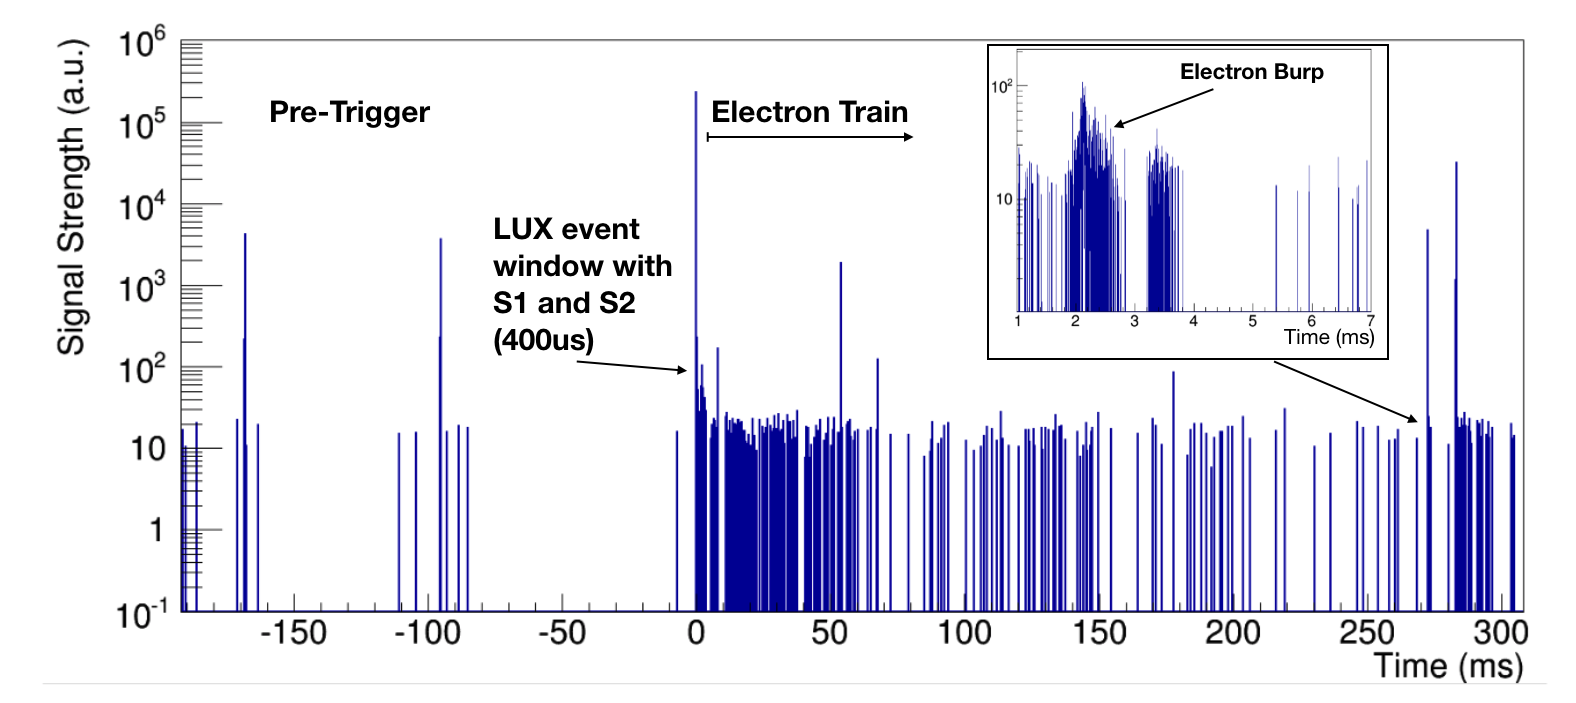
\includegraphics[width=\textwidth]{figures/etrains/lux_etrain_eburp.png}
\caption{An electron train spanning several ms. Pre-trigger and electron train regions are indicated along with the \acs{LUX} event that originated the electron train. The inset shows the shorter time structure of e-burps. The y-axis is a proxy for phd/sample. Figure courtesy of J. Xu. }
\label{fig:lux_etrain}
\end{center}
\end{figure}


In Section~\ref{sec:non_wimp_searches_with_lxetpcs}, we discussed several dark matter searches that differ from the standard \ac{WIMP} search and how they can be completed with dual-phase \ac{LXe} \ac{TPC}s. In particular, recall the Xenon10 search for low-mass \ac{WIMP}s \cite{Angle2011}. The S2-sensitive trigger threshold was set to the level of a single electron, but an analysis threshold of 4 electrons was required for S2 size. The reason behind this is illustrated in Figure~\ref{fig:xenon10_s2s}. Although single electrons following a high-energy event can be positively identified as belonging to an electron train, electron trains can last $O(10-100)$~ms. In any event window following the start of electron train, it is unknown whether the single electron is truly a small energy deposition from a low-mass dark matter event or if it belongs to an electron train. Moreover, single electrons from a train can pile up in time, creating energy depositions the size of 2 and more electrons -- so an analysis threshold of 2 electrons is not sufficient to cut out electron train backgrounds. In general, electron trains are irritating for \ac{WIMP} searches because some percentage of the detector livetime is taken up by electron train pile-up; but they greatly limit the discovery potential for low-mass searches, as the expected signal size (S2 of 2 or 3 electrons) is possibly electron train pile-up, and therefore must be considered as such.

\begin{figure}[htbp]
\begin{center}
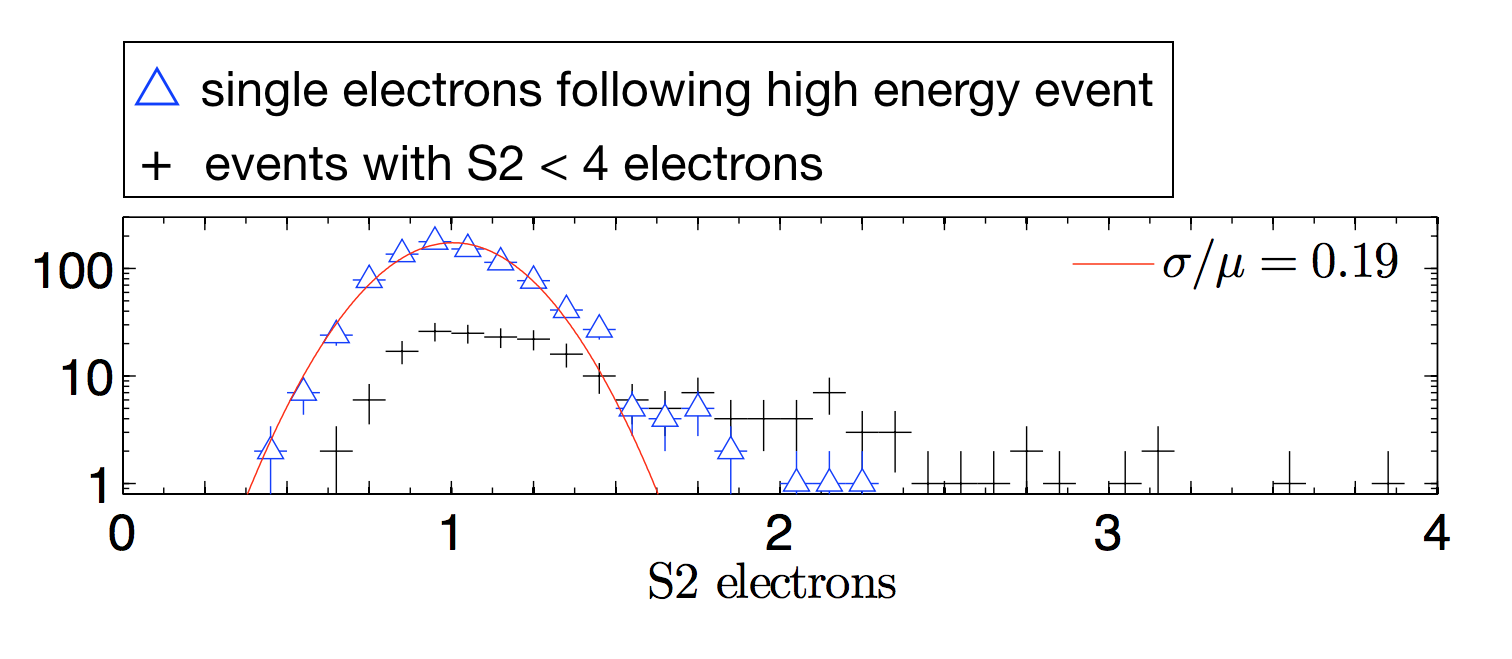
\includegraphics[width=0.9\textwidth]{figures/etrains/xenon10_s2s.png}
\caption{A histogram of the small electron signals in the Xenon10 low-mass dark matter search. The significance of the plot is that single/few-electron pluses immediately following an S2 can be positively identified as belonging to an electron train. In subsequent event windows, single electrons can appear alone or in coincidence as a small S2, which can be mistaken for the S2 produced by a low-mass dark matter interaction. Figure adapted from \cite{Angle2011}.}
\label{fig:xenon10_s2s}
\end{center}
\end{figure}

Xenon100 measured the rates of 1-,2-, and 3-electron signals following an S2 \cite{Aprile2014}. They saw a relation of the time constants $\tau_{3} \approx \tau_{1}/3$ for 3-electron signals compared to 1-electron signals, and $\tau_{2} \approx \tau_{1}/2$ for 2-electron signals. They note that if multi-electron signal results arise from accidental time coincidences of single electrons, these time relations can be explained. Quoting from \cite{Aprile2014} :

\begin{quote}
Indeed if $R_{1}$ is the rate of single electrons, the accidental time coincidence of $n$ single electrons is $R_{n} = R_{1}^{n}\cdot \Delta t^{n-1}$, where $\Delta t$ is the time coincidence window, which
corresponds to the mean S2 width ($\sim$ 1~$\mu$s).... [T]he electron rates decrease with time by following the expression $R_{n}(t) = R_{n}(0) \cdot \mathrm{exp}(- t /  \tau_{n})$. By substituting this equation in the previous formula we obtain the final relation $\tau_{n} =\tau_{1}/n$. 
%The accidental coincidence scenario is also supported by the PMT hit pattern of the multi-electron signals, which are not localized around one PMT but rather spread over the
\end{quote}

\section{Origin of Delayed Single Electron Signals}
While the origin of delayed single electron signals is still an area of active research, some behavior of electron trains are fairly well understood. An electron train can be split into two time regions: the primary event window ($O(100)$~$\mu$s, e.g. 400~$\mu$s in \ac{LUX}), and the following train, which continues for $O(10-100)$~ms. A few features are typically evident in the primary event window, which have origin in physical phenomena. These phenomena and what is found in the literature are discussed in the following subsections. The testbed study and its result, which shed more light on the origin of delayed single electron signals, are presented later in the chapter. 

\subsection{Photoionization on Grids} 
The large number of \ac{VUV} photons in big S2s are capable of liberating electrons from metallic electrodes. Electrons can be photoionized on any grid in the \ac{TPC}, but the effect is largest on the grids closest to the gas gap where the S2 is generated. Photoionized electrons from the anode aren't detected because they have essentially no space in which to proportionally scintillate. Photoionized electrons from extraction grid are directed toward the gas gap, extracted and then undergo proportional scintillation. These electrons join the S2 signal at a delay approximately equal to the distance between the extraction grid and the liquid-gas interface. Large S2s have tails that are composed of electrons photoionized from the extraction grid. An average of many high-energy S2s, clearly shows the photoionization feature (Figure~\ref{fig:s2_averages}). 

\begin{figure}[htbp]
\begin{center}
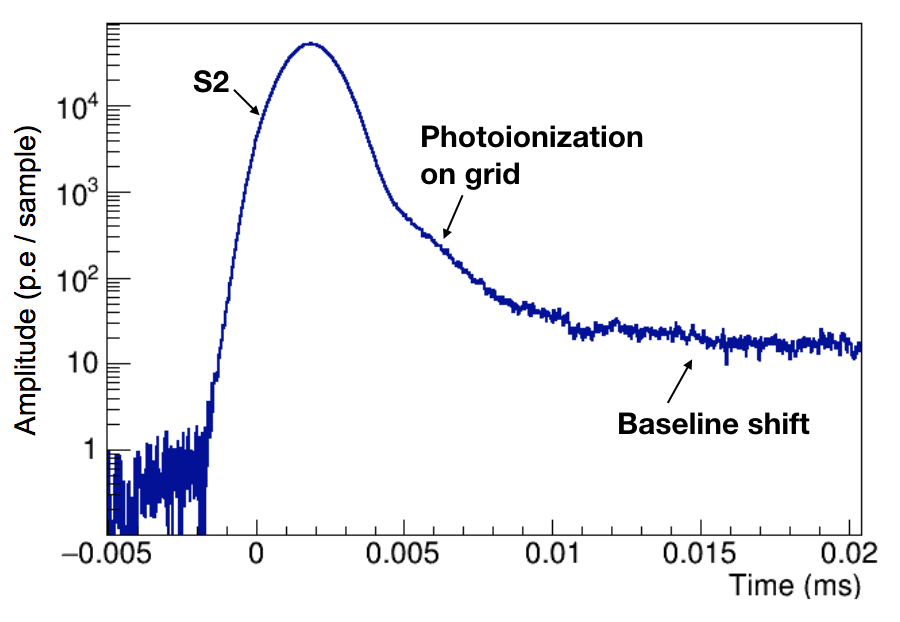
\includegraphics[width=0.8\textwidth]{figures/etrains/s2_averages.png}
\caption{The average of many high energy S2s from \acs{LUX}, plotted with logarithmic y-scale, showing a prominent photoionization feature. After the photoionization, an instrumental effect is visible: for the highest-energy events, one to a few \acs{PMT}s often do not return to baseline quickly, which gives the single electrons in the following train artificially higher areas. Figure from J. Xu. }
\label{fig:s2_averages}
\end{center}
\end{figure}


\subsection{Photoionization of Impurities} 
\label{sec:photoionization_impurities}
Electronegative impurities in the liquid (e.g. O$_{2}$) capture ionization electrons from events as they are drifted to the gas region (e.g. O$_{2}$ binds an electron at 0.45~eV to become O$^{-}_{2}$). Just as the \ac{VUV} photons can ionize electrons from grids, they can also ionize electrons attached to impurities. Xenon100 found that the rate of single electrons in the primary event window scaled with S2 size, as well as the concentration of impurities \cite{Aprile2014} (see Figure~\ref{fig:electron_rates}). Some of the electrons in the primary event window of an electron train are now believed to come from photoionized impurities. This is supported by Xenon100 data which showed that the rate of single electrons has a sharp cut off corresponding to the maximum drift time, and the the PMT hit pattern of the multi-electron signals are not localized around one PMT but rather spread over the PMT array \cite{Aprile2014}. 

\begin{figure}[htbp]
\begin{center}
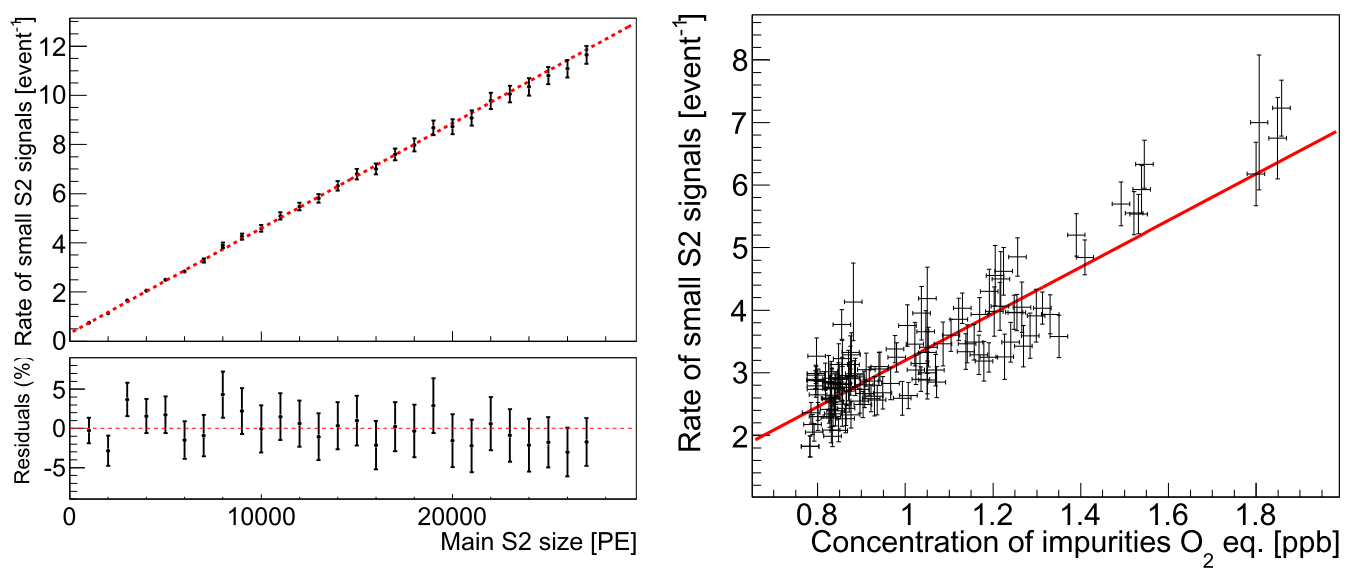
\includegraphics[width=\textwidth]{figures/etrains/electron_rates.png}
\caption{(left) The per-event rate of single electron signals 20 to 150~$\mu$s after the main S2 of a single-scatter type event as a function of the main S2 size. The fit line and residuals show a good proportionality in the relation. (right) The per-event rate of single electron signals, for events with the main S2 between 5000 and 10000 phe, as a function of the O2-equivalent concentration of impurities in liquid xenon. Figures from \cite{Aprile2014}.}
\label{fig:electron_rates}
\end{center}
\end{figure}


\subsection{Delayed Extraction of Trapped Electrons} 
Dual-phase \ac{LXe} \ac{TPC}s depend on the ability to extract electrons from liquid into gas. This is accomplished with some efficiency, called the \ac{EEE}. Gushchin et al. measured the absolute \ac{EEE} in xenon and argon in 1982 as function of electric field  \cite{Gushchin1982} (see Figure~\ref{fig:eee}. Their result extends to an extraction field of 5~kV/cm in the liquid. It is common practice for modern experiments that achieve an extraction field $\gtrsim$~5keV/cm to assume they have 100\% extraction, an assumption based on the Gushchin result. Relative extraction efficiency is measured only by the size of the S2 scintillation light and inferred number of initial ionization electrons based on calibration source energy and knowledge of recombination. Relative measurements of \ac{EEE} as a function of extraction field assume 100\% extraction at the highest field and scale the other points accordingly. In contrast, absolute extraction efficiency measurements measure the number of electrons generated in the liquid as well as how many are extracted with no scaling. 

\begin{figure}[htbp]
\begin{center}
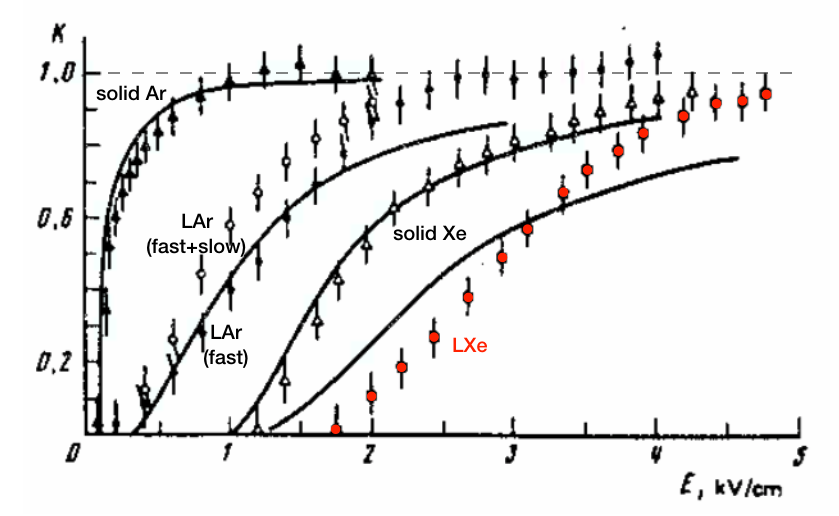
\includegraphics[width=\halffig]{figures/etrains/gushchin_eee.png}
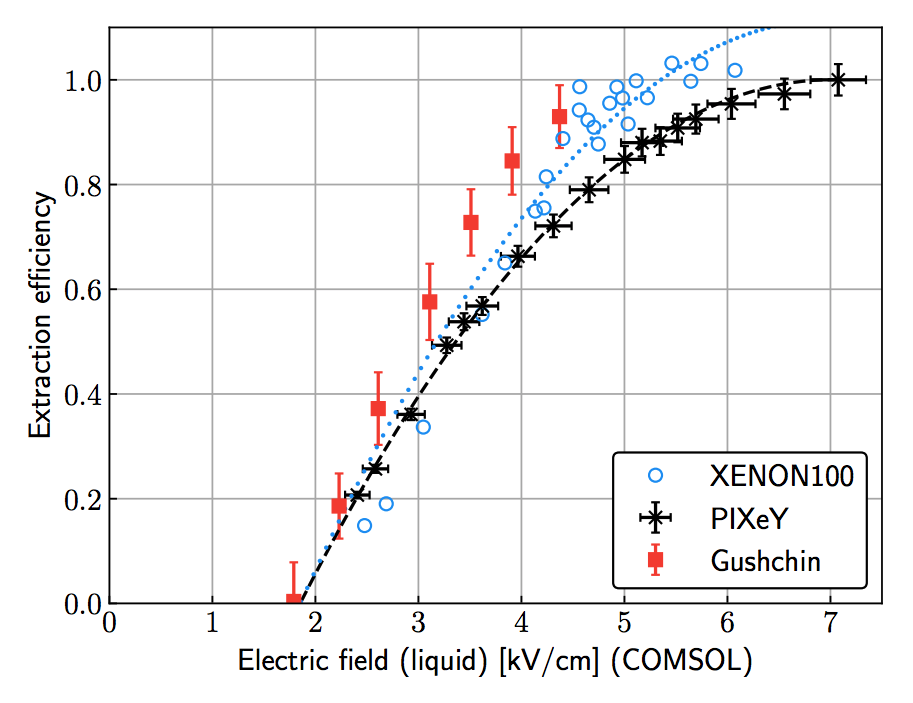
\includegraphics[width=\halffig]{figures/etrains/modern_eee.png}
\caption{(left) The absolute \acs{EEE} measured by Gushchin from \cite{Gushchin1982}. The \acs{LXe} points were re-colored red. (right) Two relative \acs{EEE} measurements from modern experiments, Xenon100 and PIXEY, compared to Gushchin. The plot is from the PIXEY result \cite{Edwards2018}, where the authors fit their result with a quadratic function ($y=ax^{2} + bx + c$). The fit to the PIXEY data (black dashed line) is scaled by a constant and applied to the Xenon100 data (blue dotted line). }
\label{fig:eee}
\end{center}
\end{figure}

Since there does not exist a second absolute measurement of \ac{EEE} out to higher extraction fields, it is uncertain when 100\% \ac{EEE} is reached in \ac{LXe}. However, it is well known that the number of extracted electrons depends on the extraction field. In addition to photoionization of impurities, it is thought that the unextracted electrons are liberated from the liquid surface at a later time, making up some component of electron trains \cite{Aprile2014}, \cite{Edwards2018}. To understand why we must consider the energy of the electrons in the liquid, and the potential barrier they encounter in order to escape into gas.

When an electron approaches a dielectric boundary held at a constant potential, a potential barrier results from its image charge. This barrier, called the Shottky barrier, takes the form \cite{Sorensen2017}:

\begin{equation}
\phi_{b} = \frac{e^{2}}{8\pi \epsilon_{0} z} \frac{\epsilon - 1}{\epsilon + 1}
\end{equation}
where $z$ is often taken to be the lattice spacing of the medium, $\epsilon$ is the dielectric constant of the medium, and $\epsilon_{0}$ is the usual vacuum permittivity. If \ac{LXe} is arranged in a simple cubic lattice, $z \approx$ 4~\AA, and the calculation yields $\phi_{b} = 0.61$~eV \cite{Sorensen2017}. The potential barrier of liquid xenon was measured by Tauchert to be 0.67~eV \cite{Tauchert1975}. There are two modes for emission of electrons across a surface boundary: (1) ``hot'' electrons accelerated by an electric field gain enough energy to overcome the barrier and be extracted (2) emission of thermal electrons, where only electrons in the tail of the velocity distribution have enough energy to escape the boundary. For an external field $E$, the Schottky barrier is lowered by \cite{Sorensen2017}:

\begin{equation}
\Delta \phi_{b} = e \Big ( \frac{eE}{4\pi \epsilon_{0} z} \frac{\epsilon - 1}{\epsilon + 1} \Big ) ^{1/2}
\end{equation}
The $E$ field also results in the aforementioned heating of the electrons. The new energy distribution $f$ can be determined by solving the Boltzmann equation as in \cite{Cohen1967}, but this is not shown here. With $f$ and adjusted barrier height, the \ac{EEE} as a function of electric field can be calculated. It is the fraction of electrons with energy expectation value above $\phi_{b} - \Delta\phi_{b}$:

\begin{equation}
\label{eq:kappa}
\kappa = \int_{\phi_{b} - \Delta\phi_{b}}^\infty K^{1/2} f(K) dK \Big / \int_{0}^{\infty} K^{1/2} f(K)dK
\end{equation}

$K = K(E)$ is the electron energy, which is implicitly a function of the electric field and $f(K)$ is the energy distribution of the electrons under the influence of an electric field. The factor within the integral is $K^{1/2}$ instead of the usual $K$ in order to select only electrons that have an upward velocity component. The red \ac{LXe} line in Gushchin's \ac{EEE} result (Figure~\ref{fig:eee} (left)) is from this calculation with the assumption that $\phi_{b}=0.61$~eV. Bolozdynya follows a similar approach and notes that electrons which are not emitted as hot electrons are thermalized by collisions and can be emitted later as thermal electrons \cite{Bolozdynya1999}. Others have treated the potential barrier as a free parameter and fit to data. Gushchin, seeing that the line did not fit the data for \ac{LXe}, treated the value of $\phi_{b}$ as free in the integral above. He found $\phi_{b}= 0.85$~eV was a better fit \cite{Gushchin1982}, but the agreement is still not very satisfying. Sorensen implemented an $n$-th chance model for electrons approaching the liquid-gas boundary, where the cumulative probability of emission after $n$ attempts is $\kappa_{n} = 1 (1-\kappa)^{n}$, where $\kappa$ is as in Equation~\ref{eq:kappa} \cite{Sorensen2017}. This reference shows that with $\phi_{b}= 0.34$~eV and $n=20$, the $n$-th chance model fits Gushchin's original data \cite{Sorensen2017}. If the $n$-th chance model is applied, with some assumptions about the relaxation time for electrons to be thermalized, the time constant for emission of thermal electrons is $O(10)$~ms. Both Bolozdynya \cite{Bolozdynya1999} and Sorensen \cite{Sorensen2017} note that the relaxation time is dependent on field (strength and direction) and temperature. Sorensen adds possible diffusion effects, fluid flow, varying surface height, etc. One critique of the $n$-th chance model is that it is unclear how the electron lifetime near the surface could be O(10)~ms, while current \ac{LXe} \ac{TPC}s achieve electron lifetimes much lower, e.g. the electron lifetime during \ac{LUX} Run03 ranged from 600-1000~$\mu$s. The argument here is that the electrons that aren't emitted should be absorbed by impurities, so they are not free to have $n$ chances of emission. Although research is still on-going into how to properly model the physics of electron extraction, there is agreement that a fast component from extracted hot electrons yields the initial S2 and a thermal component from the unextracted electrons contributes in part to the electron train.


\section{Test Bed Studies Of Electron Trains}
An initial goal of the test bed described in Chapter~\ref{ch:testbed} was to complete an absolute measurement of \ac{EEE}, since there has been so such measurement since Guschin's 1982 result. Unlike typical \ac{TPC}s, the testbed can be ``overfilled'', with the liquid level above the anode, and the generation of ionization electrons in the liquid can be measured with the charge amplifiers. The liquid level can then be dropped between the anode and extraction grid for a measure of extracted electrons with S2 (and with the charge amplifiers). During the multi-year process of instrumenting and understanding the test bed, this goal changed and evolved. In particular, it became more interesting to try and probe the source of electron trains with the hope of eventually eliminating them, rather than try to measure the \ac{EEE}. In order to provide a record, the remainder of this chapter briefly describes the attempts made with the radon source and configuration as in Chapter~\ref{ch:radon}. Finally, the most recent results published in \cite{SorensenKamdin2018}, which used the $^{210}$Po source described below, are summarized.

\subsection{Radon Source and ``Full TPC Configuration''}
\label{sec:testbed_measurement_challenges}
Here, full \ac{TPC} configuration refers to the same detector configuration as in the previous chapter (Chapter~\ref{ch:radon}); specifically, there is a 1~cm drift region and an 0.5~cm extraction region. Both cathode and extraction grids are employed. The $^{220}$Rn flow through source was initially chosen for electron train studies because of some nice properties of alpha decays. The fast chain alphas from $^{220}$Rn are:

\begin{itemize}
\item \textbf{High Energy} The alpha events in the $^{220}$Rn fast chain have energies of 6.4~MeV ($^{220}$Rn)  and 6.9~MeV ($^{216}$Po). Applying the \ac{LXe} $W$-value, shows that these alphas generate $O(500,000)$~quanta. Although ~90\% of alpha energy goes into S1 \cite{Aprile2010}, that still leaves $O(50,000)$ electrons to be detected. In contrast, a 662~keV $^{137}$Cs button source produces $O(50,000)$~quanta, but this value is $\sim$halved by recombination. Alpha light and charge yields also do not vary greatly with applied field (Figure~\ref{fig:recombination} (right)), which is convenient from an experimental standpoint of tagging a signal region and adjusting trigger conditions.  
\item \textbf{Uniformly Distributed with Compact Track} The $^{220}$Rn can be deposited directly into the \ac{LXe}, yielding a uniformly distributed source which can be fiducialized to the inner-most anode segment to avoid field edge effects. Alphas do not travel far, and so a deposition could be realistically expected to deposit all its energy in the $(x,y)$ resolution of the detector, i.e. under one and only one anode segment. This is contrast to betas, which can travel; recall the 2.2~MeV beta in the $^{220}$Rn chain that could travel 1.2~mm from Chapter~\ref{ch:radon}).
\end{itemize}

We expected to be able to select the monoenergetic alpha signal of either $^{220}$Rn or $^{216}$Po with the \ac{PMT} signal. However, \ac{PMT} saturation merged the two fast chain alphas in the S1 spectrum. There are two types of \ac{PMT} saturation effects relevant to the R8778 \ac{PMT}s used in \ac{LUX}: anode saturation and capacitor depletion \cite{Faham2014a}. The effects of the two types of saturation are shown in Figure~\ref{fig:pmt_saturation_plots}. Quoting directly from \cite{Faham2014a} to describe these two types of saturation:

\begin{itemize}
\item \textbf{Anode Saturation} The repulsive field created by a large number of electrons confined to a small spatial extent (an effect known as space-charge) yields nonlinear signal production. Since the electron cloud density is exponentially larger at the latter stages of the photomultiplier, this effect is most dominant at the anode. Anode saturation is only dependent on the instantaneous (peak) current value of the output signal. Anode saturation prevents the electron signal in the anode from further increasing. When the anode is fully saturated, the output signal cannot increase in size any further. As such, anode saturation defines the maximum peak signal that the \ac{PMT} can output. Increasing the voltage across the latter stages can provide a modest increase in anode linearity.

\item \textbf{Capacitor Depletion}  A \ac{PMT} is a current source. Due to the nature of the electron multiplication process, the signal current direction is opposite to that from the bias current. When a large signal current pulse is generated at the anode, the \ac{PMT} bias current in the last resistor decreases proportionally and the last dynode stage becomes temporarily unbiased. This effect leads to a decrease in signal size (smaller gain) and can completely turn off the multiplication process if the signal current is comparable to the bias current. A common method for mitigating the dynode voltage loss effect is to add capacitors that can provide reserve charge during a signal current pulse. These capacitors are called decoupling capacitors. Saturation effects from capacitor depletion occur when the reserve charge in the decoupling capacitors is insufficient to counteract the signal current and prevent \ac{PMT} un-biasing. Whereas anode saturation is caused by the instantaneous current, capacitor depletion is caused by the total charge drawn for a signal
 \end{itemize}

\begin{figure}[htbp]
\begin{center}
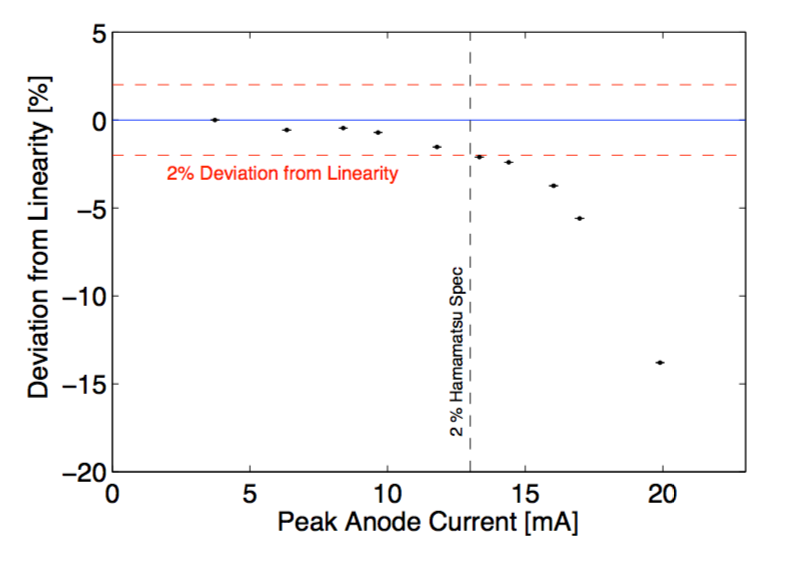
\includegraphics[width=\halffig]{figures/etrains/anode_saturation.png}
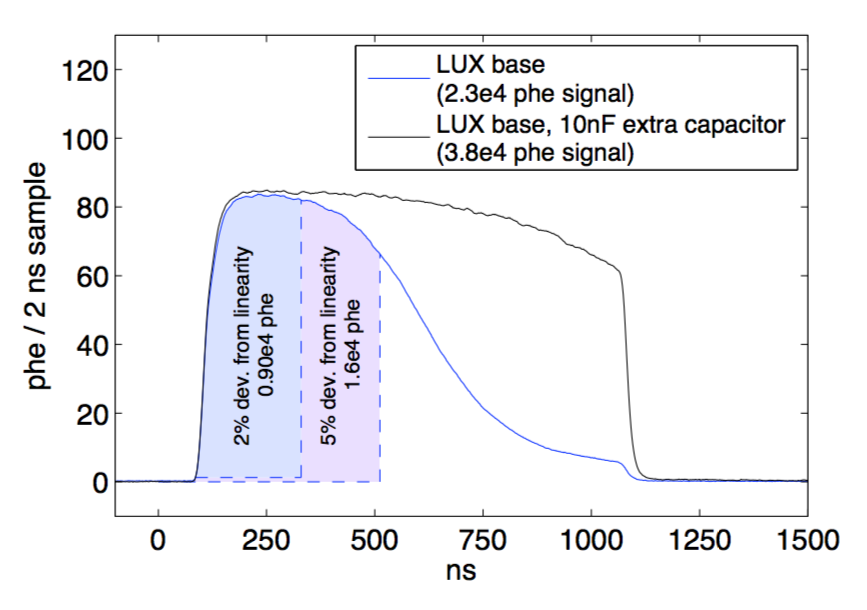
\includegraphics[width=\halffig]{figures/etrains/capacitor_depletion.png}
\caption{(left) Effect of anode saturation measured as deviation from signal linearity as a function of the peak anode current. (right) Effect of capacitor depletion on the voltage trace in the R8778. The blue trace shows the largest S2-like pulse that can be generated with a \acs{LUX} voltage divider base (generated with a 1~$\mu$s square pulse on a blue LED); the 2\% and 5\% deviations from linearity are shown. The fall-off indicates the capacitor is depleted and the photomultiplication process is temporarily turned off. The black trace shows the effect of adding an extra capacitor between dynodes Dy9-Dy10. Figures are from \cite{Faham2014a}, which also contains more information about the \acs{LUX} \acs{PMT}s and bases. }
\label{fig:pmt_saturation_plots}
\end{center}
\end{figure}

It is noted in C. Faham's thesis that any signal within 50~$\mu$s after a large pulse is also subject to non-linearity \cite{Faham2014a}; therefore, the S2 signals also did not yield a usable spectrum for separating  $^{220}$Rn from $^{216}$Po decays. Operating the \ac{PMT} at a bias voltage $\lesssim$ 1000~V resulted in less visible saturation, but single photoelectron sensitivity was lost below an operating bias voltage of $\lesssim$ 1200~V. Since single electron proportional scintillation signals are comparatively small, single phe sensitivity was desired for electron train studies. A series of masks were implemented to try reduce the overall light collection, while still retaining single phe sensitivity. Of course, on the other side, over-masking and not collecting enough photons would also result in inability to distinguish peaks. The masks are shown in Figure~\ref{fig:pmt_masks}. Initially, we started with the smallest mask and thought we had made the mistake of cutting out too many photons. However, even with the smallest mask size, which reduced the effective \ac{PMT} cathode area by $\sim$98\%, the anode current was estimated to be $\sim$50~mA, which from Figure~\ref{fig:pmt_saturation_plots} is far past where the effects of anode saturation cause loss in signal linearity. The anode current can be estimated using the following relations:

\begin{equation}
I_{PMT} \approx \frac{N_{photons} \cdot G \cdot e}{S1_{width}}
\end{equation}
where $G$ is the \ac{PMT} gain. Note that the numerator gives the charge at the \ac{PMT} anode and the $S1_{width}$ is in units of time; thus the equation above is a simple current = charge / time relation. For the 2\% mask, the highest voltage without visual saturation was 1250~mV. The single phe peak was at 35~mV/ns for that bias voltage, which corresponds to a gain of 8.7$\times$10$^{6}$. \ac{PMT} gains can be calculated by the relation:

\begin{equation}
G  = \frac{SPHE \cdot 1\times 10^{-12}} { R \cdot  e}
\end{equation}
where $SPHE$ is the pulse area of a single photoelectron in mV/ns, obtained from a spectrum of dark current pulses; an example of a single phe spectrum in Figure~\ref{fig:single_phe} shows a single phe peak at about 80~mV/ns.  $R$ is the effective output resistance of the \ac{PMT} base,  $R=25~\Omega$ for the \ac{LUX} \ac{PMT} bases \cite{Faham2014a}. The factor $1\times 10^{-12}$ reflects that the original photoelectron was amplified by the 12 dynodes of the R8778. The average alpha pulse area with the 2\% mask and and the \ac{PMT} at 1250~mV bias was 37500~mV/ns, so combining with the single phe size, $N_{photons} = 1070$. Combined with a typical $S1_{width}$ of 30~ns, this yields $I_{PMT} \sim50$~mA.

\begin{figure}[htbp]
\begin{center}
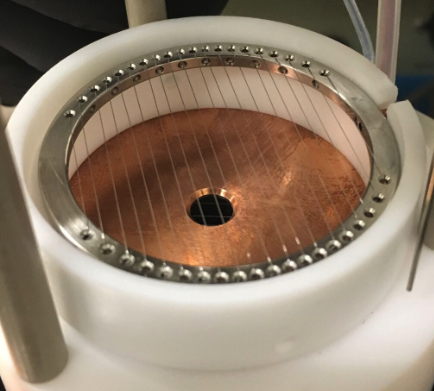
\includegraphics[width=\halffig]{figures/etrains/mask1.png}
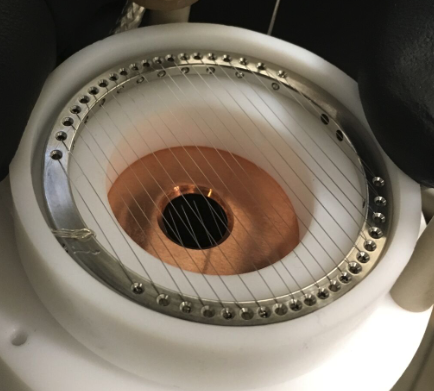
\includegraphics[width=\halffig]{figures/etrains/mask2.png}
\\
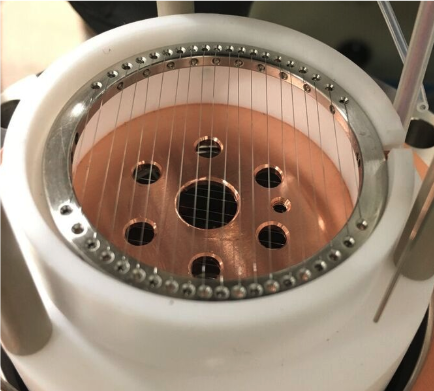
\includegraphics[width=\halffig]{figures/etrains/mask3.png}
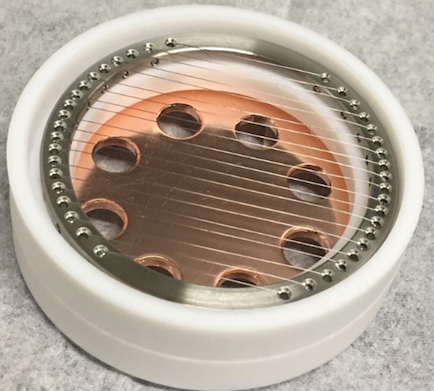
\includegraphics[width=\halffig]{figures/etrains/mask4.png}
\caption{A series of \acs{PMT} masks made from \acs{CF} blanks which reduced the light collection area of the \acs{PMT} to approximately 2\%, 5\%, 15\%, and 10\% (clock-wise from top left). The masks were installed in place of the \acs{PMT} shield grid, and similarly to the \acs{PMT} grid, they were kept at the same bias voltage of the \acs{PMT}. }
\label{fig:pmt_masks}
\end{center}
\end{figure}

\begin{figure}[htbp]
\begin{center}
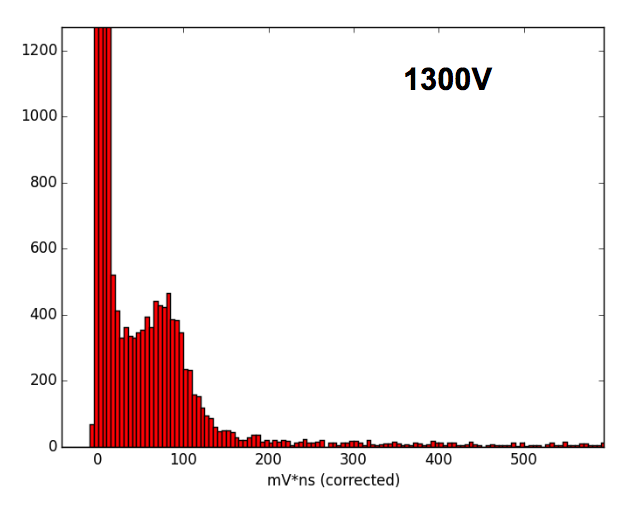
\includegraphics[width=\halffig]{figures/etrains/1300V_singlephe.png}
\caption{The single phe spectrum from the \acs{PMT} with a bias voltage of 1300~V. The spectrum was obtained by using a variable gain amplifier to 100x amplify the \acs{PMT} signal (at room temperature, in vacuum). A \acs{NIM} quad discriminator was used to externally trigger the picoscope. The waveforms were summed in a fixed window, and the results were histogrammed. The single photoelectron peak is appears around 80~mV/ns, and the double photoelectron peak is visible around 160~mV/ns. (See \cite{Faham2015} for more detail on the double photoelectron emission in \acs{VUV}-sensitive \acs{PMT}s.) }
\label{fig:single_phe}
\end{center}
\end{figure}

While \ac{PMT} saturation was the main challenge for selecting a monoenergetic source from the $^{220}$Rn fast chain alphas, geometrical signal efficiency was also an issue. The central anode segment was only 1\% of the total anode area, so most of the signal was not in this area. The radon could be distributed directly into the teflon stack (with a \ac{PTFE} tube) for a higher rate, but this increased the noise environment for the charge amplifiers. In theory the charge spectra should have had two distinct populations for the $^{220}$Rn and $^{216}$Po alphas, but with the slow trigger rate and ambient background radiation ($\beta$, $\gamma$) depositing various amounts of charge across the anode segments, two peaks could not be distinguished. A large loss in charge was also observed across the extraction grid (see Figure~\ref{fig:charge_vs_drift}), which decreased the signal to noise ratio. Bunemann's equation describes the necessary condition for grid transparency for transiting charges, i.e. it describes what relative voltages of cathode, grid, and anode result in zero electric field lines from the cathode terminating on the grid \cite{Bunemann1949} \cite{Bevilacqua2015}:

\begin{equation}
\label{eq:bune}
\frac{V_{A} - V_{G}}{V_{G} - V_{C}} \cdot \frac{D_{C-G}}{D_{G-A}} \geqslant \frac{1 + \rho [1 + \frac{d}{4\pi D_{G-A}} (\rho^{2} - 4 ln\rho) ]} {1 - \rho [1 + \frac{d}{4\pi D_{C-G}} (\rho^{2} - 4 ln\rho) ]}
\end{equation}

Where $C$ denotes cathode, $G$ denotes grid, and $A$ denotes anode. $d$ is the grid pitch, $D_{C-G}$ and $D_{G-A}$ are respectively the distances between $C$-$G$ and $G$-$A$ and $\rho$ is defined as $\rho \equiv 2\pi \frac{r}{d}$ where $r$ is the grid wire radius. The \ac{LHS} and \ac{RHS} of Equation~\ref{eq:bune} can be reorganized as: $T \equiv \mathrm{log}_{10}(LHS - RHS)$ to give the transparency condition $T \geqslant 0$. An example result, $T$ as a function of $V_{C}$, is shown in Figure~\ref{fig:bune} for a grid voltage of -4.0~kV. The charge-vs-drift plot in Figure~\ref{fig:charge_vs_drift} shows a loss of charge across the grid for voltage setting $V_{G}$ = -4.0~kVm, $V_{C}$ = -6.0~kV, and $V_{A}$ = 0V. According to Bunemann's equation plotted in Figure~\ref{fig:bune}, a cathode voltage of $V_{C}$ = -6~kV should have resulted in a transparent grid. Different voltages of $V_{C}$ were also tried, but they resulted in smaller drift fields, which reduced the charge yield from alphas. It is possible the grid transparency condition was affected by the relative angle of the cathode grid wires to those of the extraction grid; this was not investigated further.

\begin{figure}[htbp]
\begin{center}
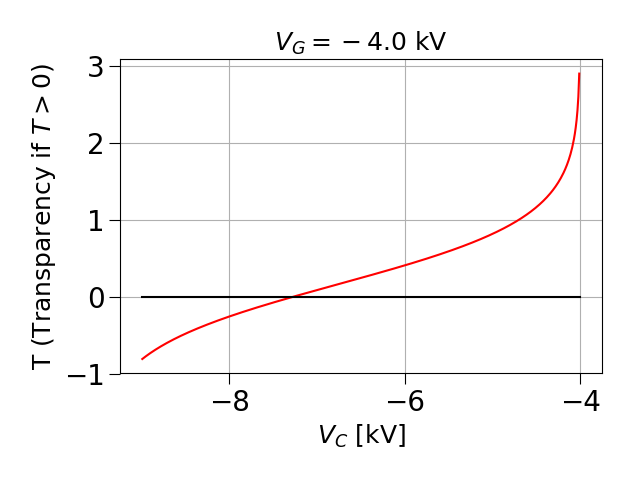
\includegraphics[width=0.7\textwidth]{figures/etrains/bune.png}
\caption{Bunemann's condition for grid transparency for a grid voltage of -4.0~kV. The cathode voltage must be between -7.24~kV and -4~kV to achieve grid transparency. A cathode voltage greater than -4~kV would result in a ``reverse field'', with the electrons drifting downward to the \acs{PMT} instead of the upward to the gas gap. For cathode voltages below -7.24~kV (more negative), field lines terminate on the grid and the charge is deposited there instead of proceeding upward to be extracted.}
\label{fig:bune}
\end{center}
\end{figure}

\begin{figure}[htbp]
\begin{center}
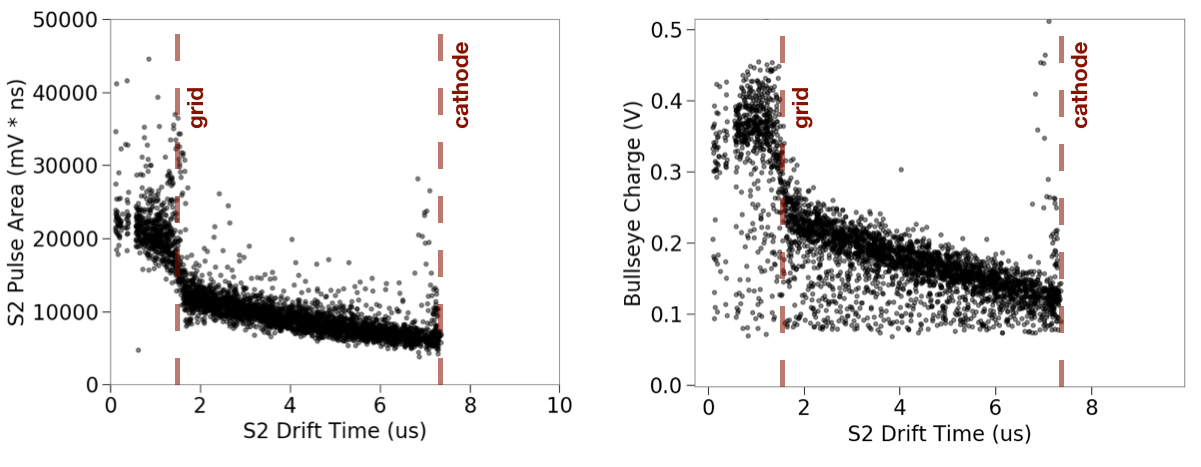
\includegraphics[width=\textwidth]{figures/etrains/s2_charge_vs_drift.png}
\caption{Ionization charge vs. drift time presented in both S2 (left) and charge amplifier voltage from the central anode segment (right). The events are $^{220}$Rn and $^{216}$Po alpha decays from the radon source. A $\sim$50\% drop in signal is visible between events occurring above the grid and events occurring below the grid. The effect of purity is also visible in the fall off of the charge signal with drift time. The points under the obvious line in the charge amplifier plot are from events which share charge with other anode segments. The charge amplifier approaches its threshold at the cathode, indicated by the sharp cut-off at 0.1~V.}
\label{fig:charge_vs_drift}
\end{center}
\end{figure}

Recall from from Chapter~\ref{ch:radon} that the late chain alphas were separable on a basis of \ac{PMT} S1 signal. The possibly of using the plated out alpha decays of $^{212}$Bi and $^{212}$Po for electron train studies was also investigated, but it was difficult to reach the purity necessary to gain a robust signal from the cathode. Note that the bullseye charge amplifier signals approach threshold level for signals from the cathode (Figure~\ref{fig:charge_vs_drift} (right)). Again, it should in theory have been possible to distinguish two peaks in the charge spectra alone, but this time there was an additional complication of the beta spectrum (recall a $^{212}$Bi beta precedes the $^{212}$Po alpha decay, this is the Bi-Po) to the issues described above. The trigger efficiency was biased to events with more charge, which made collection of a population of $^{212}$Bi alphas more difficult, and the beta spectrum polluted the charge spectrum. 


\subsection{Polonium Source and ``Extraction Region Only'' Configuration}
The grid was removed and the separation from cathode to anode was reduced to 0.5~cm. This configuration mimics the extraction region of a \ac{TPC}; there is no separate drift region. A diagram of the configuration is shown in Figure~\ref{fig:extraction_tpc}. The \ac{PMT} base was changed to an \ac{LZ} \ac{PMT} base, which has larger capacitors. However, capacitor depletion was still evident in the \ac{PMT} trace for alpha decays.  

\begin{figure}[htbp]
\begin{center}
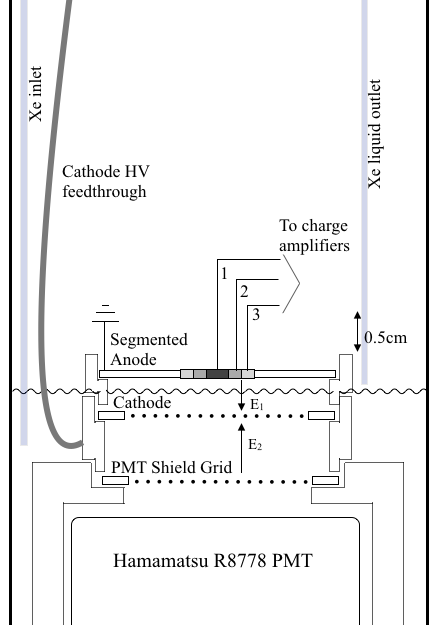
\includegraphics[width=\halffig]{figures/testbed/internals1.png}
\caption{The testbed configuration used in \cite{SorensenKamdin2018}. There is only a cathode grid and anode, with no separate drift region. The \acs{TPC} can be thought of as ``extraction region only''.}
\label{fig:extraction_tpc}
\end{center}
\end{figure}


Literature refers to the spontaneous deposition, an irreversible adsorption process, of polonium from an HCl solution on copper, silver, and nickel \cite{Hashimoto1990} \cite{Figgins1961}. A solution of aqueous $^{210}$Po (PoCl$_{4}$) was obtained and the efficacy of this process on stainless steel was tested on a $\sim$1~mm segment of the central cathode wire. A dropper was used to immerse the wire segment in the $^{210}$Po solution, and the solution was allowed to evaporate. A $\frac{1}{4}$~in blank gasket was placed under the wire to hold the drop of solution in place during evaporation (Figure~\ref{fig:polonium} (left)). The grid was then placed in the \ac{TPC} and xenon was condensed as normal. The $^{210}$Po deposition on the cathode wire was robust to dissolution in the \ac{LXe} (Figure~\ref{fig:polonium} (right)). The $^{210}$Po was also found to remain on the grid over the course of multiple fills, and the rate observed over the multiple fills ($\sim$ 3 weeks cumulative) was slightly lower than, but statistically consistent with the $^{210}$Po half-life. There were no background data sets acquired to investigate whether the few events in Figure~\ref{fig:polonium} (right) with drift times shorter than those consistent with the cathode were consistent with background. 

\begin{figure}[htbp]
\begin{center}
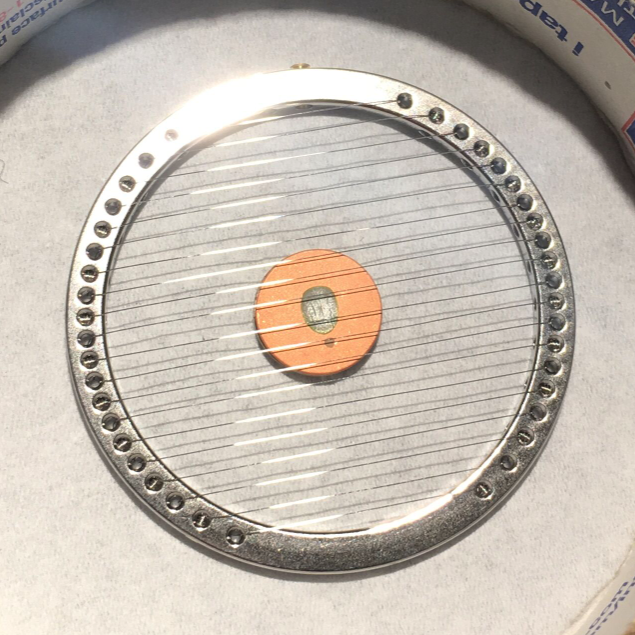
\includegraphics[width=0.3\textwidth]{figures/etrains/po_on_wires.png}
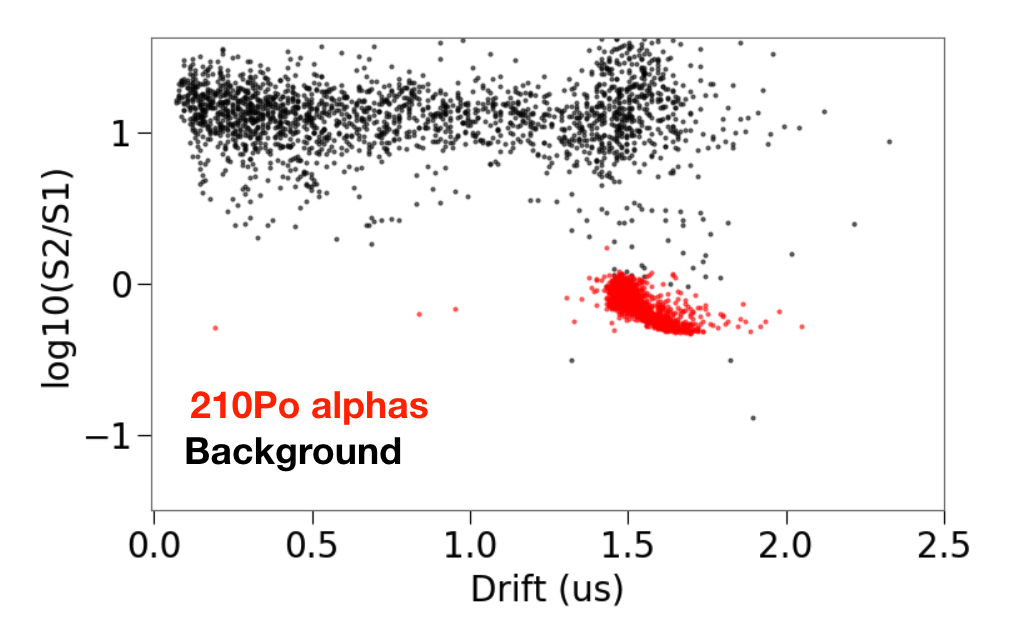
\includegraphics[width=0.6\textwidth]{figures/etrains/po_drift.png}
\caption{(left) Method for depositing $^{210}$Po on the cathode was to use a dropper to submerse a section of wire in polonium chloride and allowing the liquid to evaporate. (right) This method was robust for depositing $^{210}$Po on the cathode, as evidenced by an alpha population with drift consistent with the cathode. }
\label{fig:polonium}
\end{center}
\end{figure}


$^{210}$Po is a 5.3~MeV alpha-emitter, so it has the same high energy / many quanta generated benefit as noted above (see Figure~\ref{fig:po_decay} for a decay scheme). The deposition location was chosen to be directly under the central anode segment, which increased detection efficiency. The effect of non-uniform recombination on the grid wires is visible in polonium source, as it was visible in the plated-out radon daughters. At longer drifts, the ratio S2/S1 decreases, indicating that the decays occurred in a lower-field region (see Figure~\ref{fig:field_variation}.)

\begin{figure}[htbp]
\begin{center}
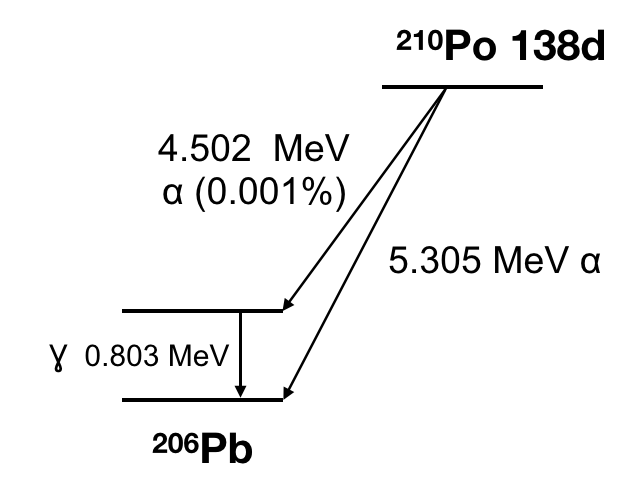
\includegraphics[width=0.7\textwidth]{figures/etrains/po_decay.png}
\caption{$^{210}$Po decay scheme. Data from \cite{LNHB}.}
\label{fig:po_decay}
\end{center}
\end{figure}

\begin{figure}[htbp]
\begin{center}
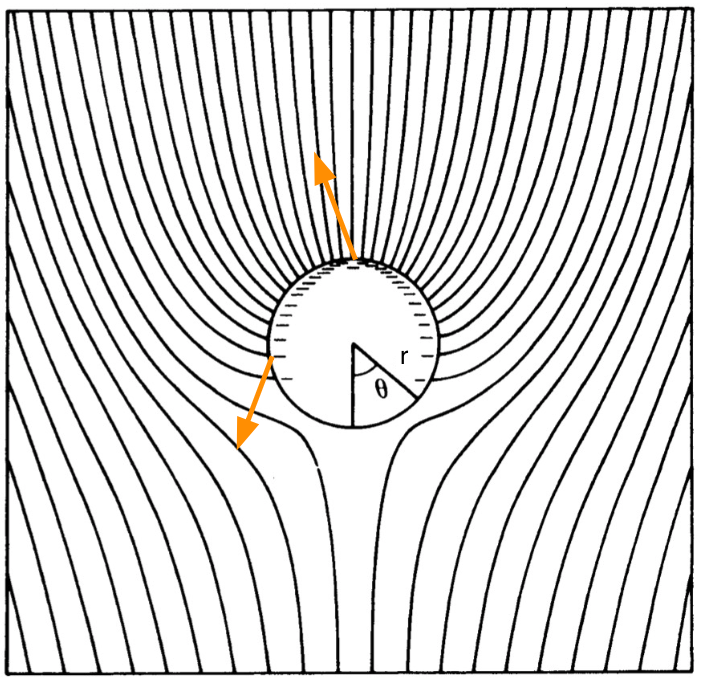
\includegraphics[width=0.4\textwidth]{figures/etrains/field_variation.png}
\caption{Decays on grid wires experience different field strength depending on particle trajectory, this results in different recombination. Adapted from \cite{Blum2008}. }
\label{fig:field_variation}
\end{center}
\end{figure}

Both $^{210}$Po alpha decay and, in the case the alpha went into the wire, recoils of the $^{206}$Pb nucleus were observable (Figure~\ref{fig:po_pbrecoil_examples}). The trigger used to observe these events was similar to that described in Chapter~\ref{ch:radon}: a coincidence between \ac{PMT} and central anode segment was required. if $^{206}$Pb recoil events were desired, the \ac{PMT} discriminator was adjusted to selectively trigger on smaller traces. As visible in Figure~\ref{fig:po_pbrecoil_examples}, the $^{210}$Po alpha provided a much richer electron train, and so these events were used in the study described in the following section.

\begin{figure}[htbp]
\begin{center}
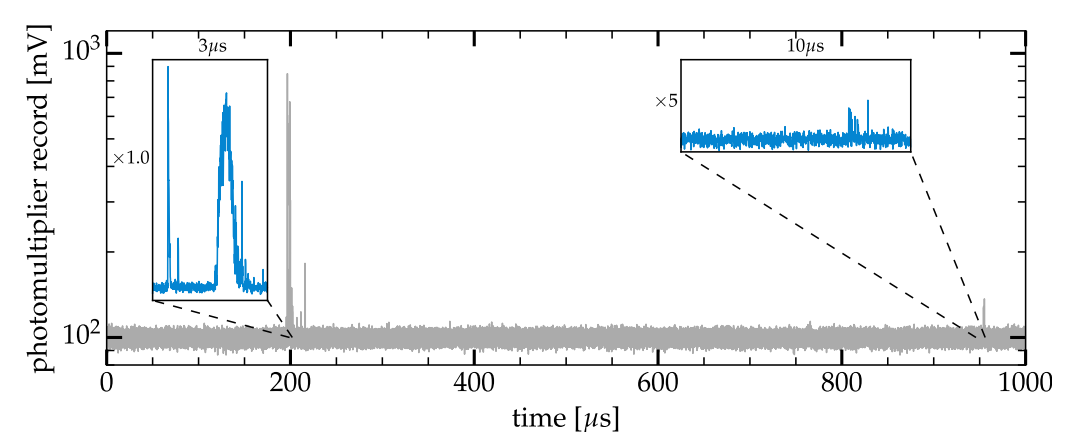
\includegraphics[width=\textwidth]{figures/etrains/event_pb_recoil.png}
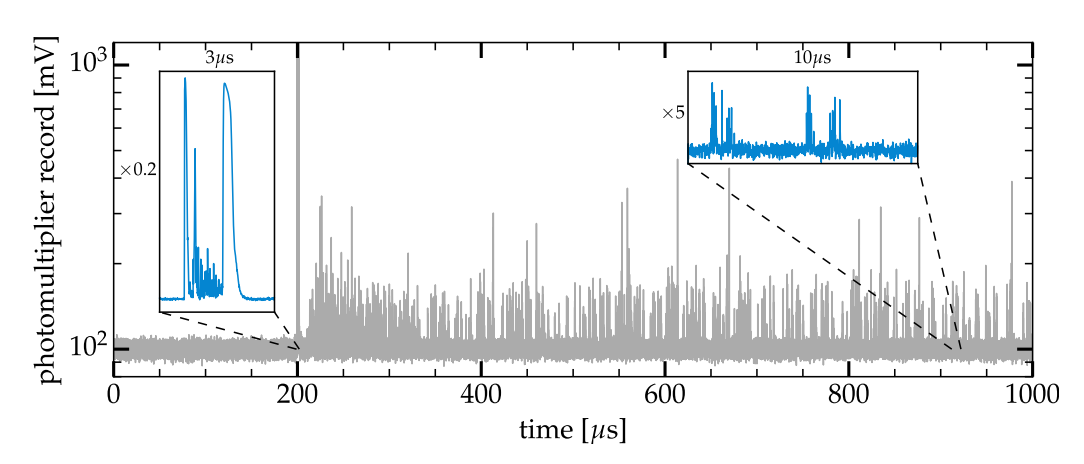
\includegraphics[width=\textwidth]{figures/etrains/event_po_alpha.png}
\caption{ (top) Recoiling $^{206}$Pb nucleus. (bottom)  $^{210}$Po alpha decay. Capacitor depletion is visible in the S2 shape, and $\sim$20~$\mu$s dead time between the S2 and start of the electron train. Insets on both (top) and (bottom) show detail of the event S1 and S2, and electron train segments. Figure from \cite{SorensenKamdin2018}. }
\label{fig:po_pbrecoil_examples}
\end{center}
\end{figure}


\section{Electron Train Study Summary}
The study done with the $^{210}$Po cathode wire source and the extraction only \ac{TPC} configuration is described in detail in \cite{SorensenKamdin2018}. Here, a short summary follows. Data were taken with cathode voltages of 3~kV, 4~kV, 5~kV, and 6~kV, and $^{210}$Po alpha events were selected. The waveforms of the events were stacked, as in Figure~\ref{fig:etrain_stack}. Two distinct time components are evident in the electron train: fast and slow. Notice the large dip in the \ac{PMT} signal followed by a rise back to the electron train -- this is the classic signature of capacitor depletion-type \ac{PMT} saturation. Due to the \ac{PMT} saturation, we were unable to observe any photoionization on grids feature following the S2.

\begin{figure}[htbp]
\begin{center}
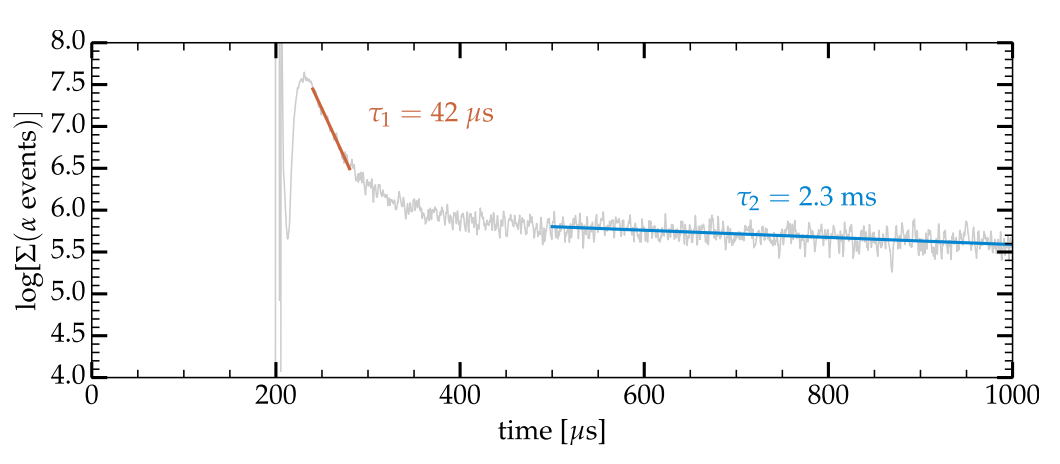
\includegraphics[width=\textwidth]{figures/etrains/etrain_stack.png}
\caption{Stacked waveforms and fits from a dataset with cathode voltage at -4~kV. Figure from \cite{SorensenKamdin2018}. }
\label{fig:etrain_stack}
\end{center}
\end{figure}

The quantity of interest is the number of electrons in each component of the electron train compared to the previous S2. Since the S2 saturates the \ac{PMT} biasing circuit capacitors, the measurement of S2 electrons is done with the charge amplifiers. It was found for \ac{PMT} voltages above $\sim$1100~V in gas or 600~V in liquid, the raw charge amplifier signal mirrored the \ac{PMT} trace (see Figure~\ref{fig:charge_reflections}). The effect was likely caused by the size of the generated at S1 and S2, which was in turn dependent on \ac{PMT} bias voltage. Two Frisch grids (cathode and \ac{PMT} shield grid) were located between the anode and the \ac{PMT} so the charge amplifiers should not have been able to ``see'' the electron cascade in the \ac{PMT}. The \ac{OV} electronics were investigated for a location where the \ac{PMT} signal could have been picked up, but none was found. The effect was likely due to pickup on the charge amplifier electronics within the \ac{IV}, as the charge signal output cables were unshielded; however, the \ac{PMT} signal output cable was shielded, with the shield at ground, so it is unclear how the signals became coupled. To solve the issue, the \ac{PMT} was merely turned off and the charge signal was acquired separately. A trigger threshold was set for the charge amplifiers with the \ac{PMT} at some low, nominal voltage (to assure we were actually selecting alpha events with the charge trigger and not background), and then the \ac{PMT} was completely turned off, and raw charge data collected.  The step height of the raw charge signals from the central anode segment were found using the step finding algorithm described in Section~\ref{sec:charge_amp_processing}. Several events were histogrammed and the mean of a gaussian fit was found and converted to the number of electrons as per the manufacturer's specifications (Figure~\ref{fig:charge_hist}). The left-skewed population visible in Figure~\ref{fig:charge_hist} is from longer drift, lower charge events that occurred in lower field regions of the cathode wires; the events were not removed before fitting the charge distribution.

\begin{figure}[htbp]
\begin{center}
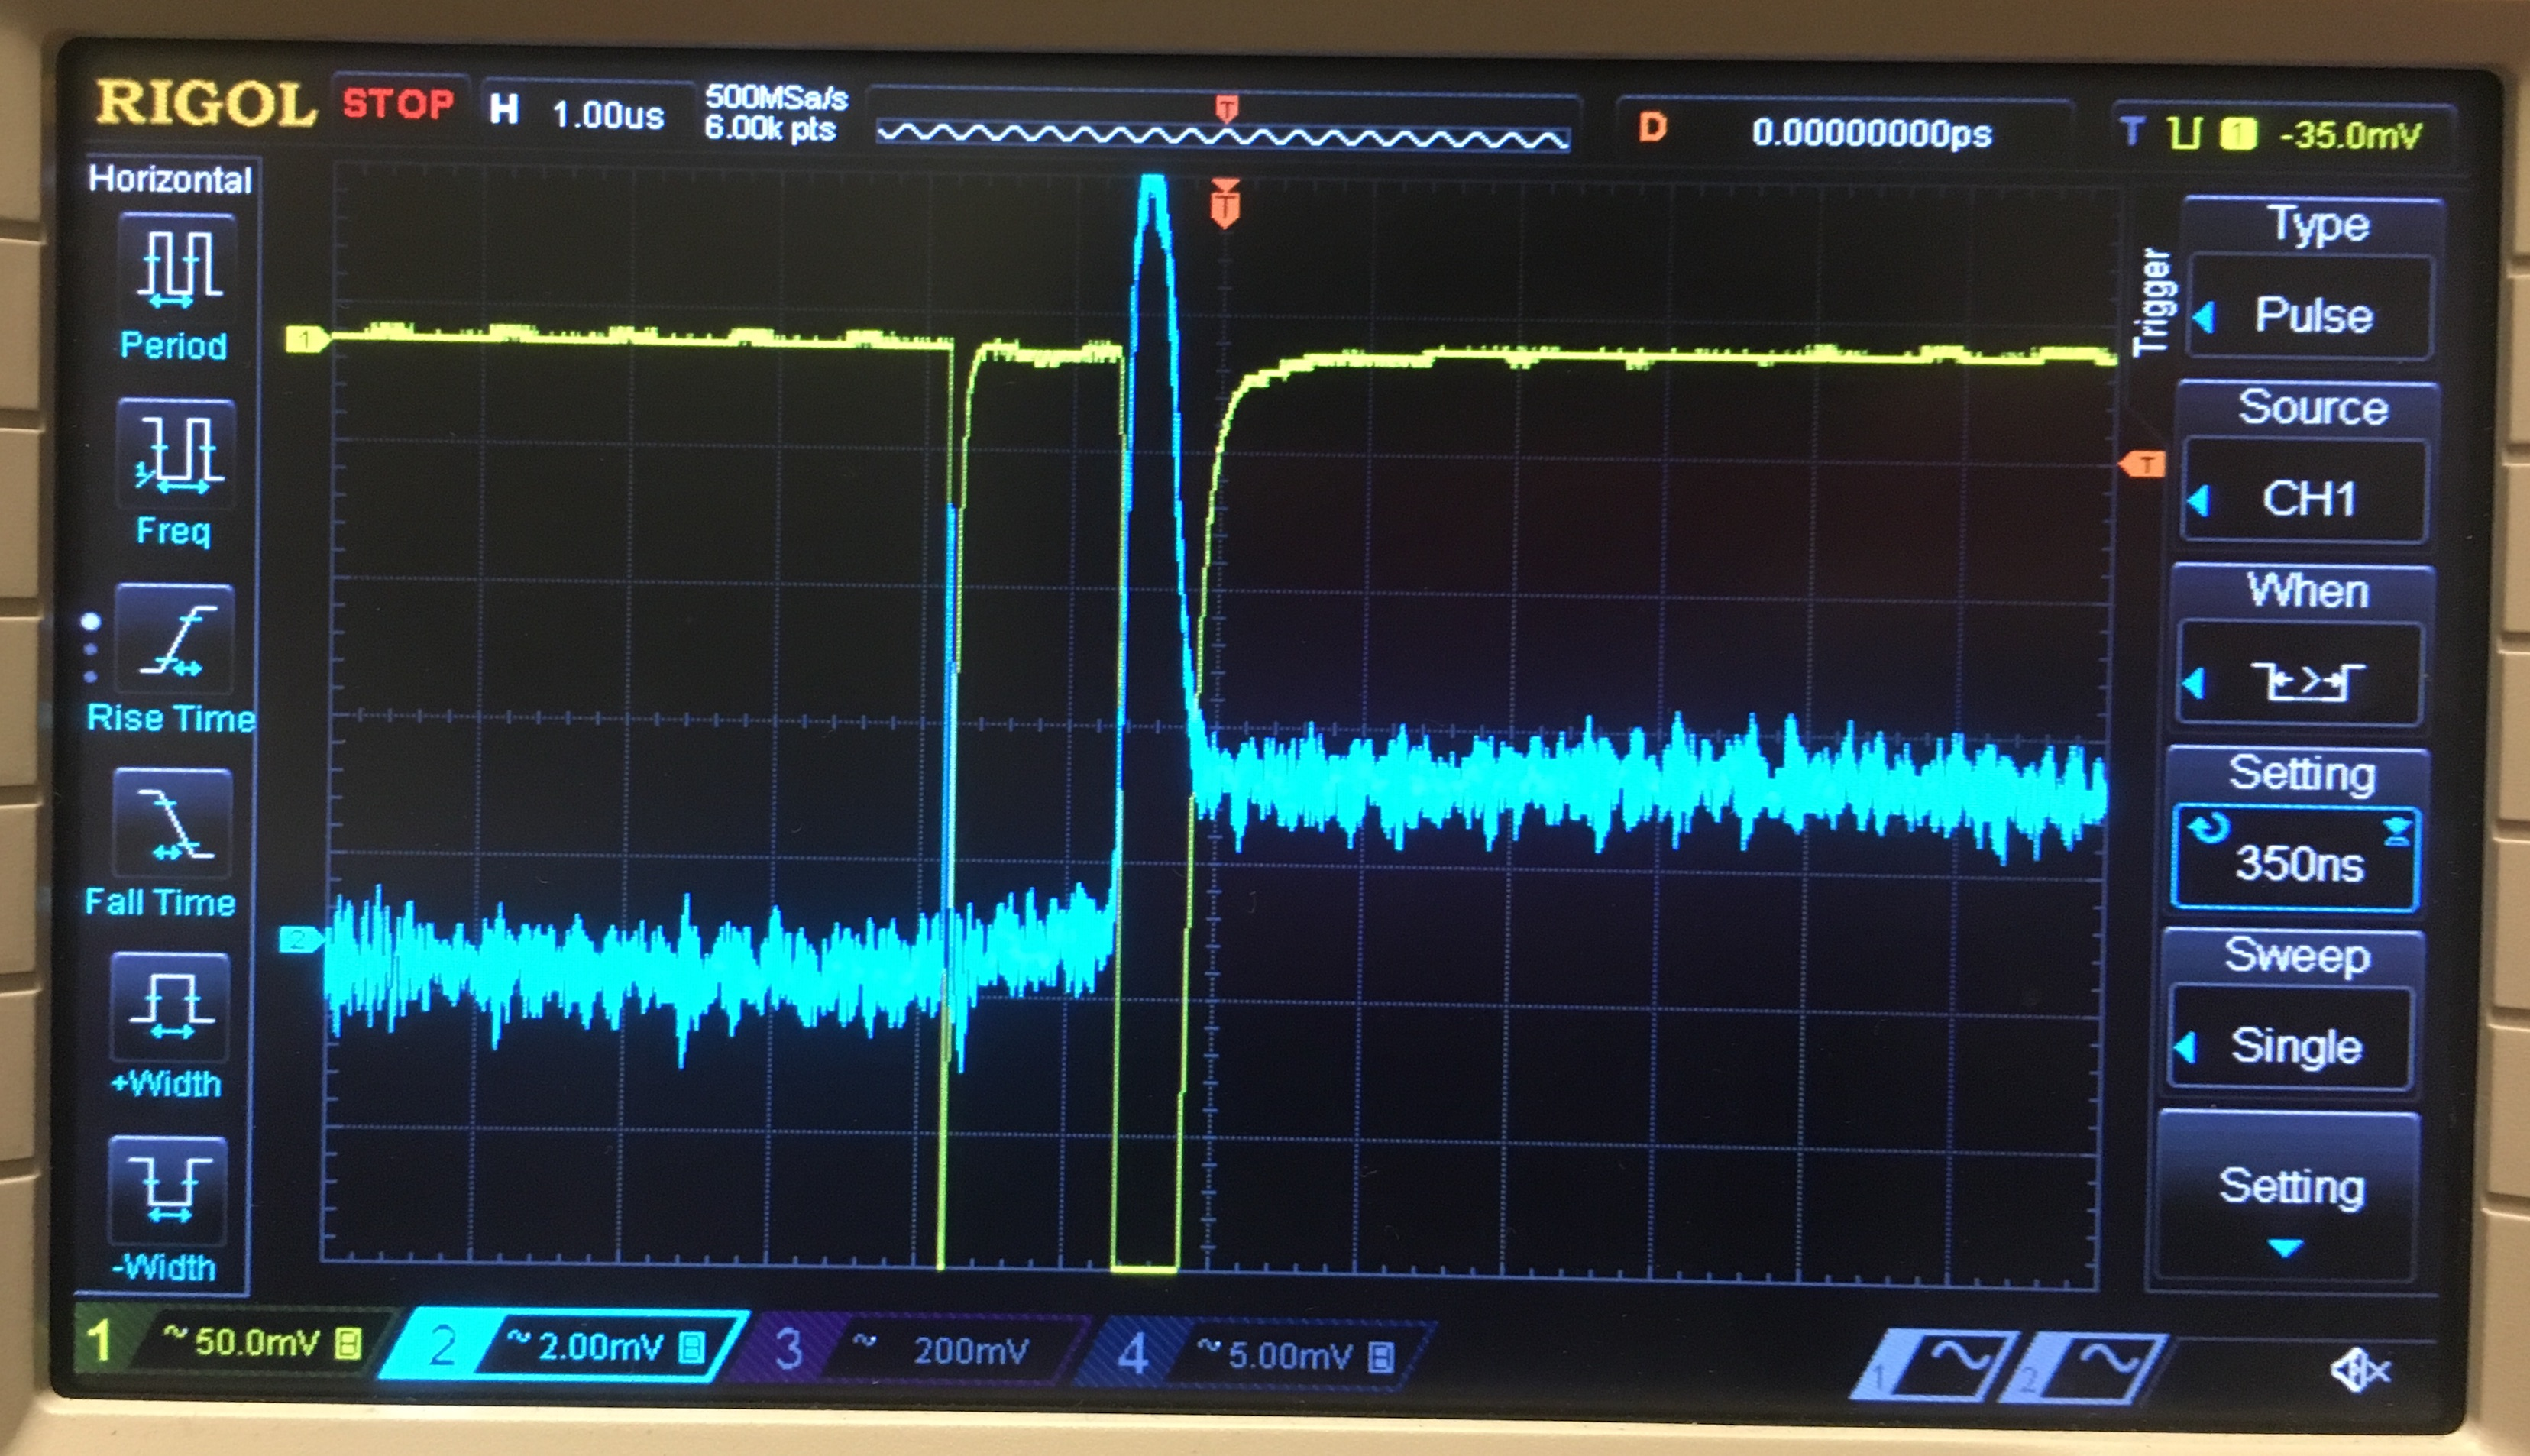
\includegraphics[width=\halffig]{figures/etrains/900V_raw_charge.jpg}
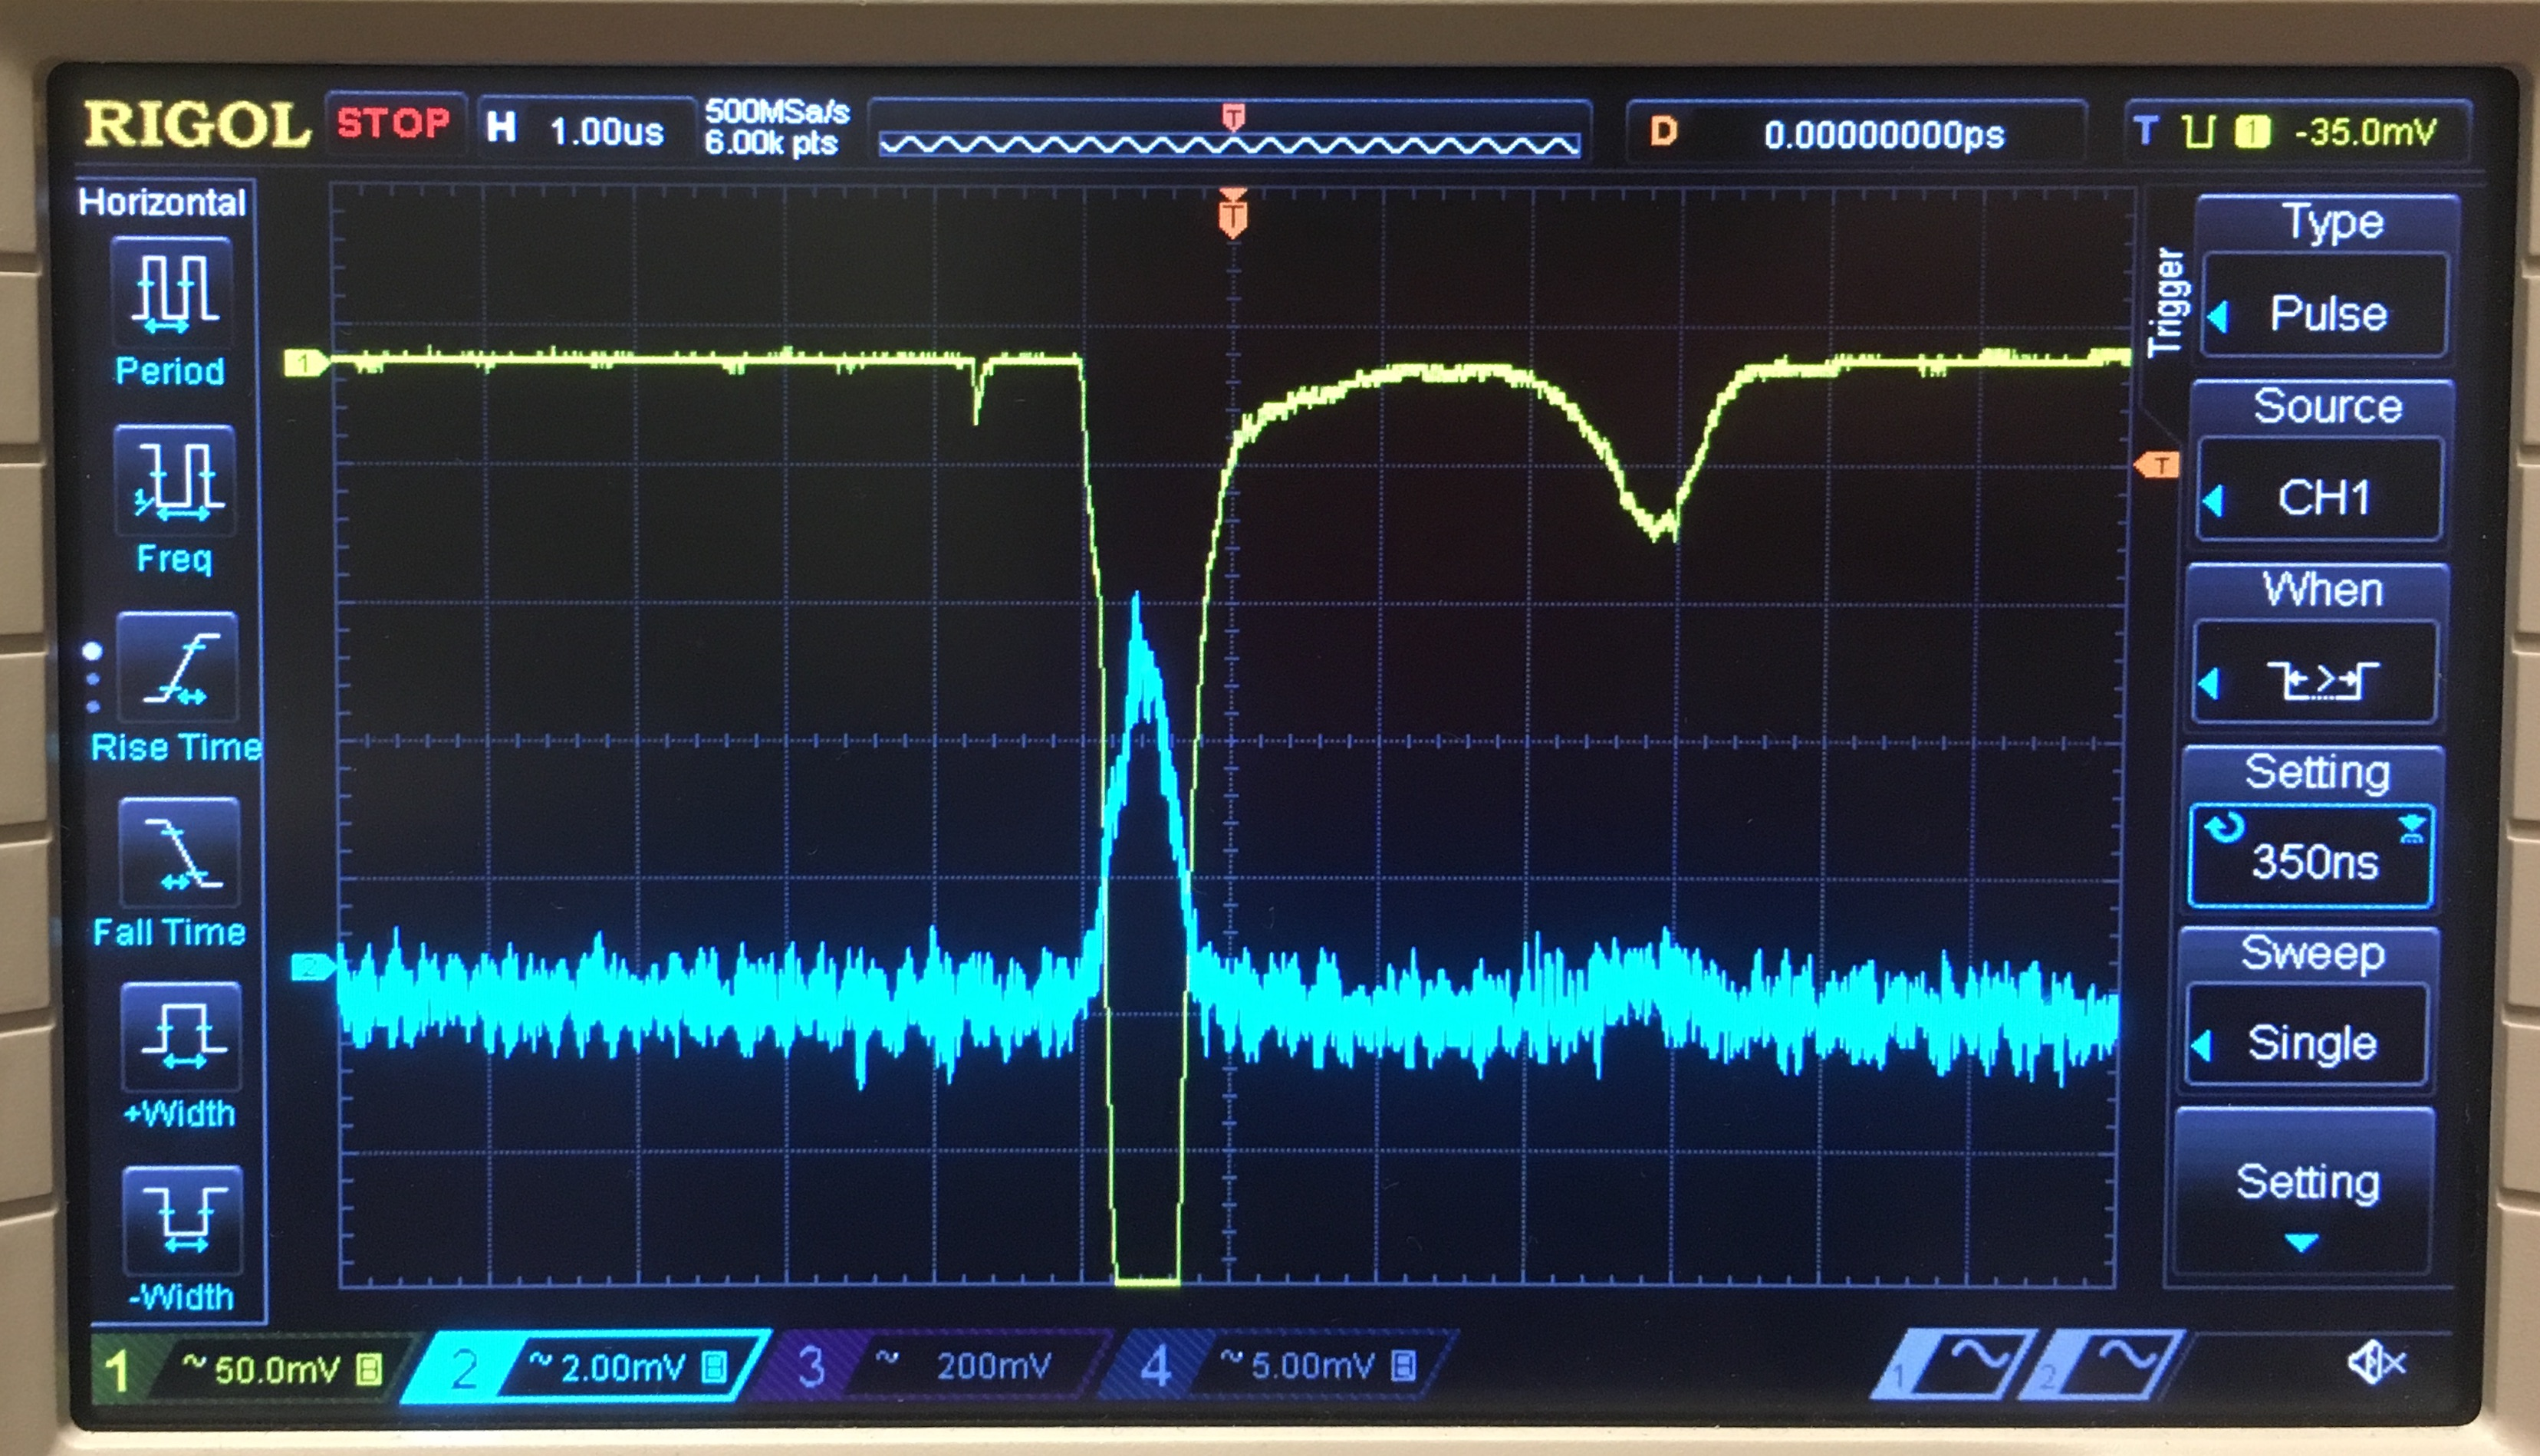
\includegraphics[width=\halffig]{figures/etrains/900V_raw_nocharge.jpg}
\caption{Examples of the charge amplifier mirror effect on one anode segment. The example (left) is an event where charge is collected on the anode segment, and so the charge amplifier signal trace shows a step. The example (right) shows the charge trace mirroring the \acs{PMT}, but with no charge collected on the anode segment.}
\label{fig:charge_reflections}
\end{center}
\end{figure}

\begin{figure}[htbp]
\begin{center}
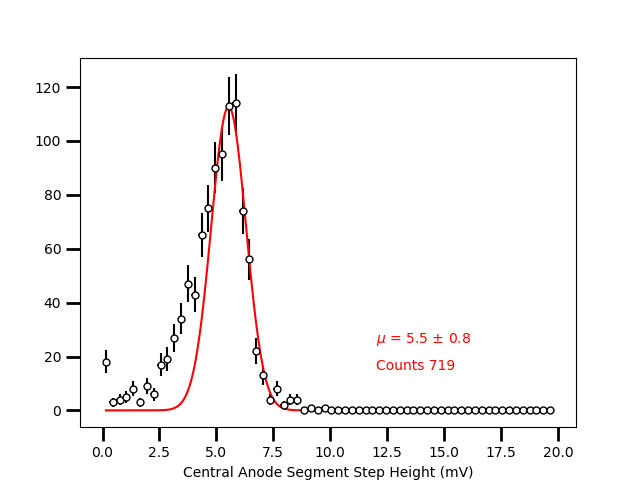
\includegraphics[width=\textwidth]{figures/etrains/charge_hist.png}
\caption{Histogram of charge amplifier step height for a cathode voltage of -3~kV. The histogram is skewed by wire position-dependent recombination; the same effect is visible in Figure~\ref{fig:polonium} (right). This mean of the fit was converted to electrons using the manufacturer's specification of charge amplifier gain, 1.4~V/pC. 5.5mV converts to 24500 electrons.}
\label{fig:charge_hist}
\end{center}
\end{figure}

The number of electrons in the train were reconstructed by summing the \ac{PMT} area above the rms-noise level, and dividing the result by the single electron size, which was measured at each cathode voltage. Based on the time constants of the fast and slow components, the number of electrons in each component was extrapolated forward to infinity and backward to the S2, correcting for the other time component. This method was preferred to pulse-funding and counting the single electrons because single electrons pile up in time, resulting in multi-electron pulses, which would have introduced a new source of error. The single electron peak was acquired with a similar method as the single photoelectron peak described above (see Figure~\ref{fig:single_phe}); the obvious difference being that the \ac{PMT} was immersed in liquid xenon and the $^{210}$Po was generating the electrons. An example of the single electron and single photoelectron peaks is shown in Figure~\ref{fig:single_e}.

\begin{figure}[htbp]
\begin{center}
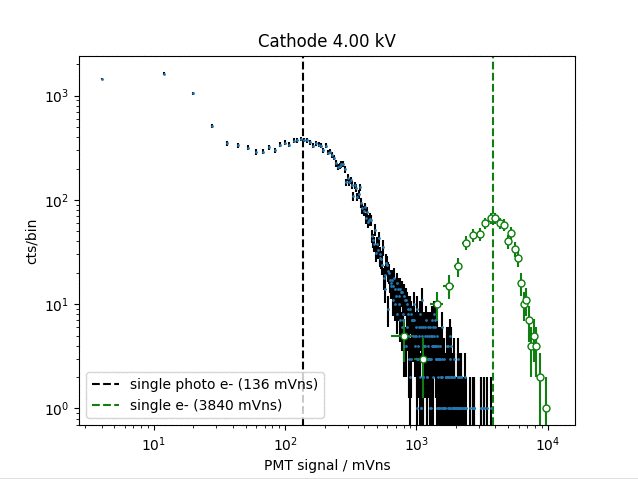
\includegraphics[width=\textwidth]{figures/etrains/single_e.png}
\caption{Single electron and photoelectron peaks obtained in liquid conditions for a \acs{PMT} bias voltage of 1500~V.}
\label{fig:single_e}
\end{center}
\end{figure}

The number of electrons in the fast and slow components found in the \ac{PMT} trace, as a fraction of the number of electrons found in the S2 via the charge amplifiers is shown in Figure~\ref{fig:etrain_result1}.


\begin{figure}[htbp]
\begin{center}
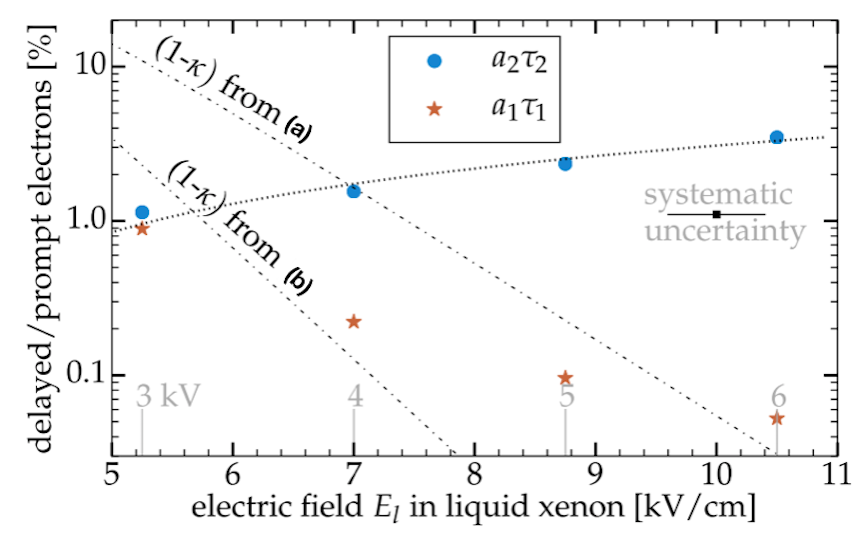
\includegraphics[width=\textwidth]{figures/etrains/etrain_result1.png}
\caption{$\kappa$ is the extraction efficiency as in Equation~\ref{eq:kappa}, so unextracted electrons should scale as ($1-\kappa$). In this thesis, (a) is reference \cite{Gushchin1982}, an absolute measurement of \acs{EEE}; (b) is reference \cite{Edwards2018}, a relative measurement of \acs{EEE}. The methods use different methods and assumptions; they are shown to illustrate that the fast component follows the behavior trend of what is expected from unextracted electrons.}
\label{fig:etrain_result1}
\end{center}
\end{figure}

The fast component of the train decreases in amplitude relative to the prompt electrons as electric field increases. This is the behavior expected if delayed extraction is the cause of electron trains. The slow component, however, increases slightly with electric field, which does not make sense if the slow part of the train has physical origin in the delayed extraction of electrons. The \ac{TPC} was left under stable operating conditions for 5 days, during which time the xenon was continuously purified through the getter. Typical flow rates were 0.2~slm, which correspond to a turn-over time of the entire liquid mass of $\sim$6 hours. The same data were acquired again, and it was found the slow amplitude decreased by a half, while the fast amplitude was unchanged (Figure~\ref{fig:etrain_result2}). The behavior of the fast and slow amplitudes with increased purity indicates that the slow component has physical origin in electronegative impurity content of the xenon.

\begin{figure}[htbp]
\begin{center}
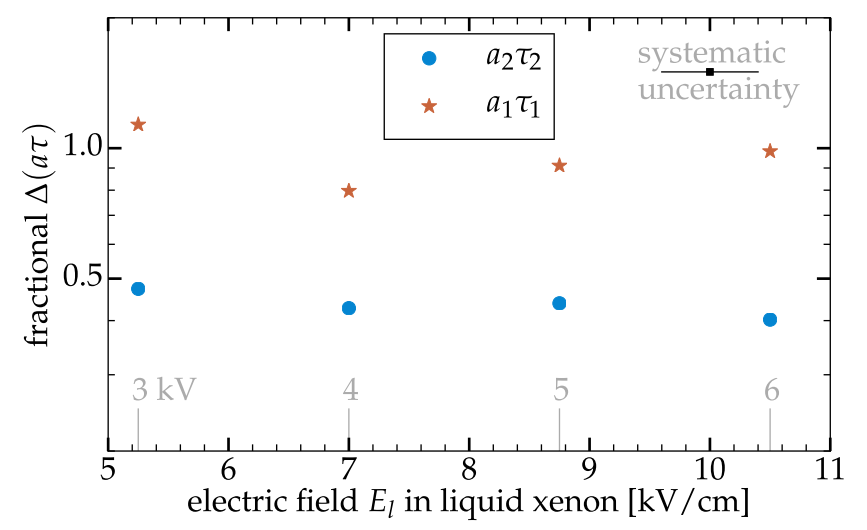
\includegraphics[width=\textwidth]{figures/etrains/etrain_result2.png}
\caption{Figure showing the ratio of fast and slow amplitude components after purification to the amplitude components measured prior to purification (shown in Figure~\ref{fig:etrain_result1}). The fast component amplitude was unaffected by the improved purity while the slow component amplitude was decreased by half with the improved purity. Note that here, as in Figure~\ref{fig:etrain_result1}, amplitudes refer to the fraction of fast and slow components with respect to the previous S2. }
\label{fig:etrain_result2}
\end{center}
\end{figure}

The time constants, themselves, were also observed to be dependent on applied electric field. This behavior is not yet understood. We found that $\tau_{1}$ = exp(2.62+0.157$E_{l}$) and $\tau_{2}$ = exp(6.32 + 0.214$E_{l}$)

\section{Discussion}
The study described in the previous section revealed two distinct time components for electron trains. The fast component amplitude decreases with increased extraction field and is not affected by purity. The drift time for the configuration of the \ac{TPC} during the study was only $\sim$2~$\mu$s, so while it is possible that photoionization of impurities was a component of the fast amplitude, it was dominated by behavior that is consistent with increasing extraction efficiency. The slow component amplitude behavior is extremely interesting: it matches the observations of delayed electron noise continuing long past a drift length in large \ac{TPC}s, and it is tied with xenon purity. This suggests the physical origin of the delayed single electrons is the release of electrons from electronegative impurities. Photoionization of impurities is one possible mechanism for liberating electrons; however, other mechanisms are also possible. Exploring the timescales of such mechanisms can help lead to a positive identification of the origin of delayed electrons. 

Electrons can be liberated from impurities by collisional detachment, tunneling, and, as already discussed, photoionization. Collisional detachment refers to the impurity's collision with other atoms, which could provide enough energy for the electron to be released. Collisional detachment can be expected to have timescales of t $\approx$ 10~s \cite{SorensenKamdin2018}, which is longer than the timescales observed in both the test bed and the larger \ac{TPC}s discussed in the beginning of the chapter. Additionally, the late time component amplitude was observed to increase slightly with a higher applied electric field, which should have no effect on collisional detachment. On the other hand, electrons tunneling out of their binding potential (0.45~eV for oxygen) should increase with applied field. However, if tunneling were the case, one would expect the timescale $\tau_{2}$ to decrease with applied field, which is counter to our observation. Photoionization of impurities by the UV xenon scintillation light has been discussed already, but other sources of light are also possible. Detector materials can fluoresce following exposure to the UV light. Fluorescence is characterized by delayed emission at a lower wavelength than was absorbed by the material. Of course, any light emitted in the visible spectrum would be seen in the \ac{PMT}, but light in the infrared spectrum would not be seen by the \ac{PMT} and is sufficient in energy to photoionize electrons from impurities. Teflon has been observed to fluoresce in the visible region \cite{Gachkovskii1969} \cite{Khatipov2011}, but this fluorescence depends on the content and synthesis of the Teflon. Other sources of fluorescing materials could be the impurities themselves. 

%One other possible source of delayed UV light is the xenon itself. Recall from Chapter~\ref{ch:LXeTPCs} that prompt scintillation light in the xenon is the result of de-excitation of the lowest bound state (singlet and triplet) of the excited xenon dimer (excimer). The excimer also has higher bound states \cite{Ermler1979}, which may decay more slowly and release UV photons, which in turn can photoionize impurities. The lifetimes of higher xenon excimer states have not been measured. It's reasonable to expect that some of the deexcitation photons of the higher bound state do not go into liberating electrons from impurities, but are instead observed directly by the \ac{PMT}. We investigated the electron trains for the presence of such single photons, but due to the close spacing of single electrons in the tail, could not distinguish for certain that single photons were not the simply result of helium after-pulsing. 

Further investigation that more closely characterizes the delayed single electron behavior with purity is planned; purity (electron lifetime) can be measured with the $^{220}$Rn source, which remains plumbed into circulation system. The \ac{PTFE} can also be removed to investigate if fluorescence of Teflon is a concern. Infrared LEDs were installed to investigate the feasibility of periodically flooding the \ac{TPC} with photons that would not interfere with the \ac{PMT} but that would be sufficient to photoionize the impurities. 



%*****************************************
%*****************************************
%*****************************************
%*****************************************
%*****************************************
